\chapter{The case of autonomous robots}
\label{ch:robots}
\vspace{-1.3cm}

The previous \Cref{ch:dua} presented the Distributed Unified Architecture, the novel framework proposed in this work. Its design and implementation have been described, from the system abstraction layer to the unit template structure. The various features and functionalities of the framework, provided by either existing tools presented in \Cref{ch:tools} or custom-made components, have been described in detail and discussed.

This work is the result of research activities spanning some years in the field of autonomous and distributed systems, as illustrated at the very beginning of this book. The Distributed Unified Architecture is the materialization of multiple attempts and ideas whose goal was to simplify research work involving autonomous systems and control architectures, as well as the activities of single developers or small teams. Many of the ideas, concepts, and requirements on which DUA is based have stemmed from long and fruitful discussions with colleagues and friends, usually held after a research project was completed, to assess what went well and what could be improved during the development process. This chapter and the next tell about the fruits of these practical experiences, showing some first applications of the DUA framework and the technologies that it integrates in real-world scenarios; their aim is to complete the comprehensive description of the proposed framework, discussing some of its notable applications and the results obtained so far by applying it to real scenarios.

Although DUA is now a general-purpose framework for distributed systems, its first versions were designed with a single application in mind, which is also the subject of this chapter: autonomous robotics. As discussed in \Cref{ch:prb,ch:tools}, autonomous robots of today are intrinsically distributed systems, from both the hardware and the software perspectives. DUA was designed to offer a unified approach to the development of such systems, providing a common ground for the integration of heterogeneous components and tools and enabling the development of sophisticated behaviors and functionalities in a modular and scalable way.

The contents of this chapter summarize the additional features that the DUA framework provides to the autonomous robotics domain, as well as the first results obtained by applying it and the technologies on which it is based to a real-world scenario. First, some robotic software packages developed for and integrated into DUA are presented. Then, to provide a concise yet explanatory example of the capabilities of the framework, two software modules developed with DUA are briefly presented: their design and development process and the challenges they posed were among the main motivations for the creation of the framework. Finally, some results obtained by applying the technologies and solutions on which DUA is based to real-world scenarios are illustrated.

\section{Software utilities for \ROS: dua-utils}
\label{sec:dua-utils}
With the system abstraction layer and the unit template finalized, a single problem is left to solve. It is of practical nature, and arises only when one starts to use the framework and, in particular, the middleware tools integrated into it for robotic software development, such as \ROS (see \Cref{sec:ros2}). The features of the \ROS middleware compose a set of services that the robotic software developer can use to build applications and modules of various degrees of complexity, and the open-source nature of the framework has allowed for a wide community to improve it over the years, reviewing existing functionalities and adding new ones. Nonetheless, the \ROS middleware is a complex system, and its many features can be overwhelming for a beginner or a developer who is not familiar with all of its functionalities. Moreover, some of its APIs are not as intuitive as one would expect, requiring complex code to be written to perform simple tasks which cover instead the vast majority of their use cases.

The \ROS community is aware of these issues, and the development effort is improving the quality of the software every day. However, over some years of experience and active development of \ROS modules, the necessity arose to create a set of utilities that would simplify some parts of the framework, wrapping its complexity and providing a more intuitive interface to the developer. While waiting to propose the same set of changes to the community and have them integrated into the official \ROS distribution, a process that can notoriously happen but also take a long time, the author preferred to develop the same set of utilities as packages that could be integrated in the system configuration provided by every DUA base unit, so that they could be immediately distributed and used in the development of robotic software modules based on DUA. Note that these software modules, as shown later on, are maintained as independent projects with no specific ties to DUA, so that every published work that uses them can be easily integrated into other systems, frameworks, or architectures for the benefit of the scientific community; this is also the case of the two example modules presented later on in this chapter.

This led to the creation of the third foundational pillar of DUA: the software collection called \texttt{dua-utils} \cite{masocco_dua-utils_nodate}. Note that, although at the time of writing it is a collection of utilities for \ROS and robotic software development, it may host different kinds of third-party software packages that can be useful in the development of distributed systems, as long as it is open-source and can be built with colcon. This can be seen as a limitation but it is only due to how it is currently integrated into DUA base units: at the very end of their setup process, the last stage clones the repository into the image filesystem and builds the packages contained in it, cleaning up build artifacts afterwards. This process has two main advantages: first, when the modules are built in this way they end up being part of the DUA base unit image, so that they can be used in the development of software modules based on DUA without the need to install them manually; secondly, the process is automated but performed at the end of every base unit, so if one of the utilities in \texttt{dua-utils} is updated the base unit image can be rebuilt by performing only this last step, reusing previous cached layers and saving time and bandwidth. What described so far may of course change in the future, should the necessity arise to include in \texttt{dua-utils} software packages that cannot be built with colcon or that simply concern other domains of distributed systems development. The motivating idea is that \texttt{dua-utils} is a way to customize the very base layer of the DUA framework which is provided to and intended for its users, who can actively suggest and modify its contents to adapt the framework to their most frequent necessities and usage scenarios.

To give an idea of the set of improvements that DUA provides to the \ROS middleware, as well as a comprehensive overview of the work that has been done so far not only with DUA but also on it, the following sections introduce some very representative utilities that are part of the \texttt{dua-utils} collection.

\subsection{Managing \ROS processes: dua\_app\_management}
\label{sec:dua_app_management}
\texttt{dua\_app\_management} is a collection of software modules and source files for the management of applications and processes in the Distributed Unified Architecture. This package contains modules, both compiled and source-only, to be included in DUA-based projects. It is particularly aimed at the development of \ROS applications, with the aim of simplifying some common tasks and wrapping boilerplate\footnote{In the context of software development, \emph{boilerplate} code refers to long code portions that must be written each time in the same way, to perform what is usually a simple and frequent operation. Programmers usually prefer either simpler APIs or wrappers, \emph{i.e.}, equivalent code items that take less options but are simpler to write, addressing the most frequent use cases.} code, especially that which involves the lifecycle of a process and requires calling the OS to do so.

The package currently contains the \texttt{ros2\_app\_manager} C++ package, which provides two libraries and the implementation of a component container (see \Cref{sec:ros2_nodes}). The first goes by the name of the package itself, and is a header-only library that implements a wrapper object for the usual main thread code of \ROS applications, \emph{i.e.}, processes that run single nodes or collections thereof or act as component containers. The necessity for this library comes from the fact that, if one wants to write the \texttt{main} function for a \ROS application going a little beyond what the examples from the official documentation show, one finds after some time that the same code is written over and over again, with only the node name and the node class changing. Operations performed by this code usually include initializing the ROS MiddleWare context, which is the entrypoint towards the underlying communication middleware used by \ROS, configuring options for the \ROS node, creating a proper executor for the application, and finally adding nodes to it and spinning it. The lifecycle of such an application ends when an asynchronous event, such a signal, occurs and it must shut down, stopping the executor and destroying all such objects in reverse order to correctly release resources and terminate middleware instances. The \texttt{ros2\_app\_manager} library provides a simple API to perform all these operations:
\begin{itemize}
  \item The constructor of the \texttt{ROS2AppManager} class does all the aforementioned initializations, as well as disabling I/O streams buffering for the current process to reduce latencies, which is a common practice in \ROS codes.
  \item The \texttt{ROS2AppManager::run} method spins the executor, and returns only when a signal is caught, which is the usual way to handle the termination of a \ROS application.
  \item The \texttt{ROS2AppManager::shutdown} method stops the executor and releases all resources as previously described.
\end{itemize}
The class is implemented as a template class whose template parameter is the \ROS executor class to use. The library also includes the relevant system headers.

Since signals are the most common way, at least on Linux systems which are the focus of DUA, to request the termination of a \ROS process, the user would benefit from a finer-grained level of control over their action. To clarify the description of what follows, let us briefly introduce the concept of POSIX signals. In operating systems design and programming, and in particular for systems that follow the POSIX standard, \emph{signals} are a way to notify asynchronous events to userspace\footnote{In this context, the term \emph{userspace} denotes application programs that are run and managed by an operating system kernel.} programs, a sort of software interrupt that can be delivered to a process by the kernel either on its own behalf or on behalf of another process, which may even do so due to the user's request. Different signals are identified by numerical codes, and represent different situations and errors. For example, when we press Ctrl-C to stop a program running in a terminal, the terminal tracks that key combination and sends the \texttt{SIGINT} signal to the process it is running, which is the default signal for interrupting a process. The process can then catch the signal and perform some cleanup operations before terminating, provided that it includes a handler for that signal in its code.

In \ROS applications, signals are not extensively used for two reasons: first, applications running on a robot should usually run as long as the robot is on, and second, they require a signal handler to be installed in the application code and some knowledge of the OS APIs. For this reason, \ROS usually handles signals by itself, which is good and handy but limiting in some cases. A first example scenario is if debugging is being performed to track a bug that crashes the applications: appropriately coded signal handlers have access to information concerning what was the memory state when the crash occurred, what kind of error occurred, what was the state of the application and of buses it was accessing, and so on. A second scenario is that of a prototype robot which is being tested, a situation in which applications are usually started and stopped via remote shells opened by users. Suppose that the robot is, \emph{e.g.}, a flying drone, and that such applications allow it to fly safely: it would not be desirable if, \emph{e.g.}, the WiFi link crashes and the drone follows as well because the shells that the applications were running within close abruptly; in this case, ignoring some signals like \texttt{SIGHUP} or \texttt{SIGPIPE} would be a good idea.

The second library of this package, called \texttt{ros2\_signal\_handler}, provides a POSIX-compliant signal handler module for \ROS applications, which replaces the default signal handler installed by the \ROS middleware. The library is a header-only one, and provides a class called \texttt{SignalHandler} implemented as a singleton\footnote{In object-oriented programming, the \emph{singleton} pattern is a software design pattern \cite{freeman_head_2020} that restricts the instantiation of a class to a singular instance within an entire application. Such instance is usually \emph{static}, \emph{i.e.}, it is created, and thus not constructed, by the compiler within the data segment of an executable and is already present in memory when the execution of the program begins.}. It uses the \texttt{sigaction} API to manage handlers, allowing fine-grained control over the signals that are caught and the actions that are performed when they are caught, and can be given access to the executor running in the application to stop it when a signal is caught. The library also includes the relevant system headers. The following methods are provided:
\begin{itemize}
  \item \texttt{SignalHandler::get\_global\_signal\_handler} returns a reference to the singleton instance of the class.
  \item \texttt{SignalHandler::init} installs the signal handler, which is a static method that must be called before any other method of the class. This handler can call user-defined functions when a signal is caught, and can be configured to ignore some signals.
  \item \texttt{SignalHandler::install} to install a handler for a specific signal.
  \item \texttt{SignalHandler::ignore} to ignore a specific signal.
  \item \texttt{SignalHandler::uninstall} to restore the default handler for a specific signal.
  \item \texttt{SignalHandler::fini} to reset the \texttt{SignalHandler} instance to its initial state and restore the default signal handlers for all signals.
\end{itemize}

All these features, although useful, would be useful only when a \ROS application is run as a standalone process, which is not the case for all robotics applications. In reality, what happens is that nodes may also be loaded into a process at run time: such process acts as a component container and nodes are denoted as components, as explained in \Cref{sec:ros2_nodes}. In this case, the container application is usually already compiled and provided as part of the \ROS installation. This is where the third part of this package comes in: the \texttt{dua\_component\_container\_mt} application. It is essentially a component container based on the \texttt{MultiThreadedExecutor} executor class, just like the standard \texttt{component\_container\_mt} provided by \ROS, but with the addition of the \texttt{ros2\_app\_manager} and \texttt{ros2\_signal\_handler} libraries. The application is intended to be used while testing \ROS components which may be dynamically loaded and unloaded at run time on real robot prototypes, thus accounting for the potential issues such as the one described in the example scenario above. For this reason, this container application uses the \texttt{SignalHandler} object to handle many signals and ignoring some of them, and the \texttt{ROS2AppManager} object to manage the lifecycle of the application.

\subsection{Handling Quality of Service in the right way: dua\_qos}
\label{sec:dua_qos}
In \Cref{sec:dds,sec:ros2}, the concept of Quality of Service (QoS) has been presented as a way to configure the behavior of the communication middleware in a distributed system. In \ROS, QoS policies are used to configure the behavior of the underlying communication middleware, being it either the DDS or Zenoh (see \Cref{sec:zenoh}) or something else, and are applied to topics to specify the reliability, durability, and other properties of the communication. The \ROS middleware provides a set of predefined QoS profiles that can be used to configure the communication, but it also allows the user to define custom QoS profiles to meet specific requirements. This system is very flexible and powerful, but often used in an inconsistent way. First, note that \ROS libraries provide default QoS profiles whose names range from \texttt{qos\_profile\_default} to \texttt{sensor\_data}, also explaining those purposes. However, these profiles as well as the rationales behind them come from the ROS 1 age, in which the communication was implemented by the middleware itself on top of UDP and TCP. Since there were mostly only these two protocols to choose from, one had almost always to distinguish between a reliable and an unreliable communication, which led to the establishment of a set of rules of thumb like, \emph{e.g.}, the common belief that data produced continuously by a sensor should be sent with a best-effort policy, since packet loss is always allowed. This is the case unless algorithms processing that data may also account for late packets, in which case a reliable policy should be preferred. Moreover, with the plethora of options that DDS QoS offers, these binary distinctions do not apply anymore. The \ROS API is quite flexible and allows the user to define custom QoS profiles, but the user is left alone to decide which profile to use and how to configure it. This can lead to inconsistent configurations across different nodes and topics, which can result in unexpected behavior and performance issues.

More configuration options imply that a finer control over the transmission policies can be achieved, accounting for an issue that ROS 1 struggled with: intrinsic difference in data types being transferred. For example, an inertial sensor may produce many samples every second but they will all correspond to small packets since they are made of a few numeric fields. Conversely, a LiDAR scan may have a lower frequency but produce large packets, since each scan is made of many points; a similar situation may arise with cameras. Reliability is not the only issue to consider: the frequency of the data, the size of the packets, the importance of the data, and the network conditions are all factors that can influence the choice of the QoS profile to use.

The \texttt{dua\_qos} library \cite{masocco_dua_qos_nodate} provides API that return QoS profiles that account for these issues, distinguishing first between the desired reliability of the communication and then between the data type being transferred. The repository contains two software libraries: \texttt{dua\_qos\_cpp} for the C++ language and \texttt{dua\_qos\_py} for the Python language. Apart from their actual implementation, whose details concern only the syntax of each language, the functionalities they offer are the same. Before going further, note that DUA does not enforce the use of these QoS profiles in any way nor place: they are only included as a suggestion for the user to simplify the development of \ROS applications, and are also designed to be compatible as much as possible with the QoS policies that are both provided by the \ROS middleware and used in the majority of the \ROS software available today. Lastly, the profiles are intended to be used only with topics. One can modify QoS for internal communications of services and actions too, but that is usually not recommended: those primitives are synchronous and reliable by nature and, in the case of actions, require specific QoS policies to achieve stateful communication. For these reasons, the \texttt{dua\_qos} libraries provide only QoS profiles for topics.

The first two categories are \texttt{Reliable} and \texttt{BestEffort}: these map to two distinct libraries in both packages, whose contents are almost the same. The difference they enforce is the \texttt{ReliabilityPolicyKind}, \emph{i.e.}, the reliability part of the QoS policies provided by each library. There is no additional distinction between the two categories since it is actually up to the user to decide which one to use: today, the \texttt{Reliable} category applies to practically every transmission since network congestion and bandwidth optimization are managed independently by the communication middleware used by \ROS, mainly thanks to the \texttt{HistoryPolicy}. This policy is set to \texttt{KEEP\_LAST} by default, which means that only a fixed-size buffer of samples is kept in memory to be either sent or received, and that the rest is discarded, independently of the configured reliability which comes into play shortly after, when samples are actually being transmitted; this mechanism, although not sophisticated, acts as a sort of congestion control that works well in most cases. All APIs in the \texttt{dua\_qos} libraries allow to set the depth of such buffers, but provide a default value that is usually good enough for most cases.

For each package, both \texttt{Reliable} and \texttt{BestEffort} libraries then provide QoS profiles via the following APIs:
\begin{itemize}
  \item \texttt{get\_datum\_qos}: returns a QoS profile for generic data, \emph{i.e.}, data that is not particularly large in size or requires special handling on the QoS size. This is due to the above reasoning, thanks to which both commands and setpoints, and sensor data are, \emph{e.g.}, the same thing.
  \item \texttt{get\_scan\_qos}: returns a QoS profile for LiDAR scans, spatial scans, or similar data. The peculiarity of this data is that while it may have relatively high or low frequencies, it gets easily very large in size, so a low history depth is suggested here to minimize the risk of network congestion and memory exhaustion.
  \item \texttt{get\_image\_qos}: returns a QoS profile for images, whose size may vary from small to very large, but whose frequency rarely exceeds a few tens of Hertz. The history depth default value is not as low as for scans, but still lower than for generic data and configurable by the user.
\end{itemize}
The only difference among the two libraries is that the \texttt{Reliable} one also provides the \texttt{get\_persistent\_qos}, a particular type of policy intended for reliable transmissions that may be resumed at a later point in time. This is possible thanks to a feature of the DDS standard called the \texttt{DurabilityPolicy}, discussed in \Cref{sec:dds}, which allows a publisher to store all samples in a persistent storage and send them again them when a new subscriber appears. This is useful for data that may not be produced continuously but is still important, like configuration data or state information, and is used in this library together with a higher history depth to ensure that all samples are stored and sent.

\subsection{Improving node development: params\_manager, dua\_node}
\label{sec:params_manager_dua_node}
Among the many \ROS features (see \Cref{sec:ros2}), there is one of paramount important concerning the nodes: the possibility of specifying configurable variables for them that can be inspected and set at any point in time, known as \emph{node parameters}. These parameters are usually set at launch time, either by the user or by the launch system via configuration files, and are then read by the node to configure its behavior. The \ROS middleware provides a set of APIs to manage these parameters, whose task is that of building and storing in each node a database of the parameters that it has. The keys used in this database are strings, which contain the name of a parameter. Each parameter is then associated with its type, which can be a string, an integer, a floating-point number, a boolean, or a list of any of these types, and its current value. There are also other flags and fields, identifying whether a parameter is read-only or, in case it is of numeric type, its valid ranges.

\ROS configuration files allow the user to specify only parameter values, meaning that all the aforementioned information must be provided when the parameter is \emph{declared}. In \ROS code, a \emph{parameter declaration} is the act of calling an API that creates an entry into the parameter database of the node, writing all such information which is passed as arguments to the API. To correctly declare parameters passing all the correct and relevant information, one has to write quite the quantity of code. This is not a problem when the number of parameters is small, but it can become cumbersome when the number of parameters grows, especially if they are of different types and have different constraints. As mentioned earlier, this is a classic example of boilerplate code.

Another issue concerns parameter updates and their usage in the actual code of the node. Each time a parameter must be read, the node must call an API that retrieves the parameter from the database, and then cast it to the correct type. This is not a great concern if the parameter is read only once or with a low frequency but when it is, \emph{e.g.}, the gain of a control law that must be evaluated at each high-frequency iteration of a control loop, the overhead of the database queries might become significant. Assuming that the parameter type is never going to change, something that the \ROS APIs allow but is seldom necessary in practice, it would be preferable to store the parameter value in the node and update it only when the parameter is updated. This way, parameter reads would be much faster. To achieve this, a callback must be registered with the \ROS node that is called when an update is requested for a set of parameters: when this happens, some checks like the range of the parameter have already been performed but other ones like the type of the parameter have not. Moreover, there can be only one such callback in a node, which means that it must check for which parameter an update has been requested and act accordingly.

The amount of code that one has to write to achieve the aforementioned functionalities, in every \ROS software and every time in the same way, grows uncontrollably with respect to the amount of parameters that each node has. The code that manages parameters in a \ROS node becomes unnecessarily long and complex, difficult to manage and debug. This is the motivation behind the development of the \texttt{params\_manager} package \cite{masocco_params_manager_nodate}, which provides a set of utilities to simplify the management of parameters in \ROS nodes. This package currently contains only an implementation for C++.

Before the \texttt{params\_manager} C++ library comes into play, there is a Python script that can be used to automatically generate the code that declares the parameters in the \ROS node class. This script is automatically called by a CMake directive that extends the ament installation (see \Cref{sec:ros2_buildsys}). Thus, the first step, as shown in the documentation of \cite{masocco_params_manager_nodate}, is to add a YAML file to the source code of the node that, with a specific syntax shown in \Cref{lst:paramsmanager}, contains the list of parameters that the node must manage together with all their metadata. The script will then parse this file and generate a C++ source file that gets added to the build process, containing a routine called \texttt{init\_parameters} that declares all parameters in the node and sets up the update callback. To make this work, a bit of code must be added to the node class, as shown in the documentation: a \texttt{Manager} object must be instantiated as a member of the node class, and the \texttt{init\_parameters} function must be declared as a method of the node and called in its constructor, better if at its beginning since from that point on all parameters will have been declared, set, and ready for usage. This way, the boilerplate code is reduced to a bare minimum of five lines, and all relevant parameter data must be written in a configuration file which is much easier to manage and debug than the code itself.
\begin{center}
\begin{minipage}[t]{.9\textwidth}
\begin{lstlisting}[caption={Example of \texttt{params\_manager} YAML configuration file \cite{masocco_params_manager_nodate}.}, label={lst:paramsmanager}]
header_include_path: dir/node_header.hpp
namespace: node_namespace # This is optional
manager_name: manager # This is optional
node_class_name: MyNode

params:
  camera_offset:
    type: double
    default_value: 0.1
    min_value: 0.0
    max_value: 0.5
    step: 0.0
    description: "Distance between camera and drone center."
    constraints: "Must be in meters."
    read_only: false
    validator: function_name3 # This is optional

  hsv_from:
    type: integer_array
    default_value:
      - 0
      - 1
    min_value: 0
    max_value: 255
    step: 1
    description: "HSV color lower range."
    constraints: "."
    read_only: false
    var_name: hsv_from_ # This is optional
\end{lstlisting}
\end{minipage}
\end{center}

\Cref{lst:paramsmanager} shows also two other useful features of the \texttt{params\_manager} package. The first is the possibility to specify a \emph{validator} routine or a variable name: the autogenerated parameter update callback checks the name and type of a parameter and, if a match is found, may perform other operations before approving the update. One of these is to perform an additional check, whose outcome decides if the parameter update is approved, which may be coded by the user in a function whose name is specified in the YAML file, informally referred to as a \emph{validator}. Alternatively, to account for the necessity to quickly store the new value directly inside the node as explained above, the user can specify the name of a variable member of the node class that the callback will access and overwrite with the new parameter value. Of course, the two things can be done at the same time: it is up to the user in the first case to code the variable member update inside the validator routine. To keep track of each parameter's metadata together with these two additional values, the \texttt{params\_manager} library uses the \texttt{std::set} data structure from the \texttt{<set>} C++ standard library header, which is implemented as a red-black tree for maximum efficiency \cite{guibas_dichromatic_1978}.

After the \texttt{params\_manager} library was implemented and successfully tested, the question arose whether it would be possible to eliminate the necessity of the user to write the five lines of code that instantiate the \texttt{Manager} object, call the \texttt{init\_parameters} function in the node constructor, and then clear the \texttt{Manager} at the end. Hiding the management of the \texttt{Manager} would be possible in case the base \ROS node class that each node is derived from already included an object of the \texttt{Manager} class as a variable member. In the \texttt{dua\_node} package \cite{masocco_dua_node_nodate}, an alternative \ROS base node class is provided that includes the \texttt{Manager} object and handles its lifecycle together with that of the node. This way, the only necessary lines of code to manage parameters in a \ROS node are those that declare and call the \texttt{init\_parameters} function; this is due to the fact that, by the current implementation, \texttt{init\_parameters} is a member function of the derived class and can only be called by its constructor, after the base class one has run. The \texttt{dua\_node} package is intended to be used in conjunction with the \texttt{params\_manager} package, and is included in the \texttt{dua-utils} collection.

\subsection{Wrapping clients: simple\_serviceclient, simple\_actionclient}
\label{sec:simple_serviceclient_actionclient}
\Cref{sec:ros2} presented ROS, in both its first and second version, as a project aimed at providing a middleware to robotic software developers that offers many services, the most important of which is distributed communication. To this end, \ROS provides three communication primitives: topics, services, and actions. The last two are synchronous communication primitives, meant to implement client-server communication over a short time span in the former case, and a possibly longer one in the latter case, with the additional feature of being stateful. The \ROS middleware provides APIs to create and manage services and actions, which are grouped in the server and client sides. Servers are usually simple to implement: the user instantiates the server object and defines the relevant callbacks for it. In the case of actions there are usually multiple callbacks involved, to account for every possible asynchronous event requested by the client or terminal state (see \Cref{fig:ros2act,fig:ros2goalfsm}), but the developer can choose which ones to implement based on which features of the communication their code shall actually support.

For both services and actions, the client side is instead a completely different beast. In both C++ and Python, client-side APIs are based on asynchronous programming, which is a programming paradigm that allows the user to perform multiple tasks concurrently, without the need to wait for the completion of one before starting the next. This is achieved by using callbacks together with \emph{futures}, which can be essentially described as variables whose value becomes available at a later point in time. Things get increasingly complicated as one steps from service clients to action clients, so this is the order in which the two situations are addressed here.

The developer writing code making use of a service client must first instantiate such object, then send a service request through it. The result of this API call is a future, which will eventually hold the value of the service response. The developer can act in three ways here, all made possible by the \ROS API: they can block and synchronously wait for the future to get a value, they can attach a callback to the future that will be called when the value is available, or they can poll the future at any time they want in the code and check for its value. The API to manage each of these cases is not particularly complex, but it can get quite verbose. As for all the previous sections describing packages of \texttt{dua\_utils}, the next one is motivated by a necessity that arises when one writes actual \ROS software: in the vast majority of cases, if you call a service, you need the response data right after, and you need it to be available before the next line of code is executed. This is why the first eventuality among the three described above is the most common, but it still requires the developer to write a lot of code to manage the future, put the node in a synchronous wait state by spinning an executor, and then get the value from the future. This is the reason why the \texttt{simple\_serviceclient} package \cite{masocco_simple_serviceclient_nodate} was developed.

This package offers two equivalent libraries for both C++ and Python, which offer the same methods with the exact same signatures in both languages. The libraries implement a client class that wraps the original \ROS service client, extending its functionalities. Since the other situations are better handled with the official \ROS APIs, the \texttt{simple\_serviceclient} libraries offer only two methods:
\begin{itemize}
  \item \texttt{call\_sync}: this method sends a service request and waits for the response, returning it when it is available. The method is blocking, and takes a flag argument telling whether the node must be added to an executor or not; this is to support the situation in which the node is already added to an executor and callbacks execute in separate threads, so waiting for the future consists in blocking the calling thread waiting for it to get a value using the future object API. In both scenarios, the only code that can execute while the future is being waited for is node callbacks.
  \item \texttt{call\_async}: this method sends a service request and returns a future that will hold the response when it is available. The method is non-blocking, and provided for convenience.
\end{itemize}
In C++, these libraries contain template classes whose template parameter is the type of service, so that the code can automatically handle the service request and response types.

The wider variety of cases that the stateful communication provided by actions defines is the main reason behind the complexity of its client-side. Essentially, each operation that the client requests to the server is implemented as a service call, and must be treated in the code in a way similar to what has been described before, \emph{i.e.}, using futures and eventually callbacks. Note that even the most desirable outcome for an action from the perspective of the client, \emph{i.e.}, completing a goal, requires two service calls: one to request the acceptance of the goal and one to request and get back the result (see, again, \Cref{fig:ros2goalfsm}). This easily leads again not only to a lot of boilerplate code, but also to complex code that is difficult to manage and debug. Moreover, there is an additional problem: the \ROS action API is not as well organized as the service API, due to its history. It has been one of the last features to be ported, regarding the communication services, from ROS 1 to \ROS, and its implementation is as such split among two sets of libraries: the language client library, that is \texttt{rclcpp} for C++ and \texttt{rclpy} for Python, and the \texttt{rclcpp\_action} and \texttt{rclpy.action} libraries. This dichotomy, still unresolved, has led to a situation in which the style of the client API might differ even significantly between its different parts, which reduces clarity and increases the learning curve for the developer. One of the most evident examples of this is the numerous types that are involved in client-side action programming, which model goals, their handles, futures, feedbacks, etc., and their signatures do not follow a consistent style. The API is very powerful and allows one to achieve very complex asynchronous, event-based behaviors to handle scenarios of various degrees of complexity, but the problem is the same as before. In reality, there are mostly two ways in which actions are called: either the client sends a goal and waits immediately after for the result, or the client sends a goal and then either polls for the result or requests a goal cancellation. The \texttt{simple\_actionclient} package \cite{masocco_simple_actionclient_nodate} was developed to address these issues, providing an action client class that acts as a wrapper for the original action client. The package contains again two libraries, one for C++ and one for Python, whose contents and implementations are the same. For simplicity, the following explanation will refer only to the C++ library, which implements a template class.

The first big improvement of this class over the original API is that it completely hides all the type definitions that are required to handle an action client: the only template parameter is the action type. This leads to a very simple instantiation of an action client, where all type definitions are handled internally by the class. The class constructor can also take feedback callback as argument, to be called when feedback messages are received from the server. Then, the class implements three sets of methods, whose names are self-explanatory and that implement the most important moments of an action call lifecycle. For each, this library also provides both synchronous and asynchronous variants, which counts to six methods in total:
\begin{itemize}
  \item \texttt{send\_goal}: sends a goal to the server, and returns a future that will hold the result of the goal request.
  \item \texttt{send\_goal\_sync}: sends a goal to the server, and returns the result of the goal request.
  \item \texttt{cancel}: cancels the goal that is passed as argument and returns a future that will hold the result of the goal cancellation.
  \item \texttt{cancel\_sync}: cancels the goal that is passed as argument, and returns the result of the goal cancellation.
  \item \texttt{get\_result}: requests the result of the goal that is passed as argument, and returns a future that will hold the result of the goal.
  \item \texttt{get\_result\_sync}: requests the result of the goal that is passed as argument, and returns the result of the goal.
\end{itemize}

Finally, the \texttt{simple\_actionclient} library also provides a method to handle the entire lifecycle of an action call in one go, from the goal request to the reception of the result: the \texttt{call\_sync} method. The signature of this method for the C++ library is shown in \Cref{lst:callsync}. The first thing to note about it are its arguments: apart from the goal to send, it takes a flag and a series of timeouts. The flag tells the method whether to cancel the goal if a timeout occurs, and the timeouts are the maximum time that the method will wait for the goal request to be sent, for the result to be received, and for the goal to be cancelled. The method returns a tuple, implemented in C++ with the \texttt{std::tuple} standard library class, with three elements:
\begin{itemize}
  \item a boolean flag that tells if the goal has been accepted or not by the server;
  \item a \texttt{ResultCode} object, which is an enumeration defined in the \texttt{rclcpp\_action} library that tells the result of the goal request, \emph{e.g.}, if the goal has been accepted, rejected, or cancelled;
  \item a shared pointer to the result of the goal, which can be valid or not depending on whether it was returned by the server, and that has type \texttt{ActionResultT} which is derived from the action type, the template parameter of the class.
\end{itemize}
Internally, the method performs each step by requesting each operation to the server and then synchronously waiting for the response, spinning the node. As the call progresses, the method checks for timeouts and cancels the goal if necessary, handling all possible outcomes and return values. When the return value of this method is accessed, by the way it is designed as a tuple holding the three values discussed above, the caller can immediately determine how the action call went since those three values together encode every possible outcome of the sequence of operations that the method performs. This method is the most powerful and flexible of the library, and is intended to be used in the vast majority of cases where an action is called. The other methods are provided for convenience, and to allow the user to handle each step of the action call lifecycle separately if needed. For more advanced use cases, the original \ROS API is again the best choice.
\begin{center}
\begin{minipage}[t]{.9\textwidth}
\begin{lstlisting}[caption={Signature of the \texttt{Client::call\_sync} class method from the C++ action client wrapper library \texttt{simple\_actionclient\_cpp} \cite{masocco_simple_actionclient_nodate}.}, label={lst:callsync}]
std::tuple<bool,rclcpp_action::ResultCode,std::shared_ptr<ActionResultT>>
  call_sync(
    const typename ActionT::Goal & goal_msg,
    bool cancel_on_timeout = false,
    int64_t send_goal_timeout_msec = 0,
    int64_t get_result_timeout_msec = 0,
    int64_t cancel_timeout_msec = 0);
\end{lstlisting}
\end{minipage}
\end{center}

\subsection{Implementing \ROS automata: transitions\_ros}
\label{sec:transitions_ros}
As illustrated in \Cref{sec:prb_design_challenges}, the software that operates a complex robot typically follows a hierarchical organization. The lower levels usually consist of firmware, controllers, and device drivers. More advanced modules rely on the abstractions provided by these lower layers to perform sophisticated operations. At the top, a single module typically acts as a coordinator, ensuring the proper functioning of the entire system and offering interfaces to human operators. This module usually requires complete access to the software stack of the robot for control purposes, and its design must be sophisticated enough to handle the diverse situations that might arise during the execution of the prescribed tasks that the robot must perform. The higher the level of autonomy required, the more complex this kind of software is going to be.

Finite-state machines (FSMs) are a renowned tool in computer science \cite{wagner_modeling_2006}: their mathematical foundation derived from graph theory describes a system whose behavior is represented by a sequence of discrete configurations within a finite set, called \emph{states}. These states are interconnected by a collection of \emph{transitions}, which may lead to another state or loop over the same one. Transitions occur when specific conditions are met, which alter the current state of the machine. FSMs have been widely utilized in modeling various hardware and software systems, ranging from basic algorithms and communication protocols \cite{brand_communicating_1983} to digital control systems \cite{sklyarov_hierarchical_1999, pola_symbolic_2016} and distributed systems \cite{schneider_implementing_1990}.

Before moving forward, it is essential to clarify the type of FSM relevant to this use case. In software engineering, two main categories of FSMs are recognized. The first category, often referred to as a \emph{passive} FSM, is the more commonly used of the two. This type mainly serves as an internal representation of the state of an object or algorithm, acting as a data structure that holds information about the current state without performing any actions. Methods that interact with a passive FSM are called externally and their primary role is to keep a record of the execution state of the program based on the information encoded within it. The module presented in this section focuses on the second category of FSM, known as an \emph{active} FSM. Unlike its passive counterpart, an active FSM is an autonomous entity that retains state information and actively executes operations on data and interfaces with other system components by calling appropriate APIs. An active FSM plays a crucial role in autonomous robotics by governing the behavior of the robot. This includes decision-making processes, executing movement commands, and interpreting data from its various subsystems. It is one of the most widely used paradigms for developing supervisory software for autonomous robots, as it provides a structured approach to managing the complexity of the robot's behavior; it is not the only one though, since its limitations start to show up when the automaton's complexity grows and a more modular and intrinsically nested structure would be preferable, such as behavior trees \cite{iovino_survey_2022}.

This discussion clarifies that, when looking forward to develop a supervisory software for an autonomous robot that can be modeled as a finite-state machine, an active FSM is the most appropriate choice. Moreover, if the software running on the robot is based on \ROS, having an active FSM implementation which is designed to directly support \ROS communication primitives and other middleware functionalities would be highly beneficial. The \texttt{transitions\_ros} package \cite{masocco_transitions_ros_2022} was developed to address this need: it provides the implementation of an active FSM capable of seamless interaction with \ROS software, thereby enabling sophisticated autonomous control functionalities. Such an active FSM is intended to facilitate high-level autonomy in robotic systems, allowing them to operate effectively in dynamic environments by integrating sensory inputs, executing control logic, and interfacing with other modules cohesively.

When dealing with a \ROS-based robot, one can broadly isolate three types of tasks that an automaton must handle:
\begin{itemize}
  \item \textbf{Asynchronous:} the robot must react to some external events that do not alter its state but require data processing, \emph{e.g.}, detecting a target.
  \item \textbf{Synchronous:} the robot must execute operations specific to its current state, \emph{e.g.}, arming, takeoff, landing, or exploring the environment.
  \item \textbf{Collaborative:} the robot must perform complex operations requiring real-time coordination with another agent or human operator.
\end{itemize}
Given the three communication primitives offered by \ROS (see \Cref{sec:ros2}), a logical approach for implementing a \ROS-enabled FSM would be to handle asynchronous tasks through appropriate topic subscription callbacks. In contrast, services and actions would be ideal to manage synchronous and collaborative tasks. The FSM implementation should thus include a reference to a \ROS node object, acting as a communication endpoint towards the middleware. To ensure the FSM is active in the sense described above, each state should be associated with a specific \emph{routine}, \emph{i.e.}, a function executed upon entry to the state, whose return value determines the subsequent transition. Furthermore, the FSM object should provide a \texttt{run} method that, when invoked by a running thread, sets the automaton in motion within the context of the calling thread, and returns control only once a terminal state is reached and no further transitions are possible.

The \texttt{transitions} \cite{yarkoni_transitions_2017} Python library is one of the most famous and versatile open-source software libraries that implements a finite-state machine. It has many standard features of software FSM implementations, such as support for hierarchical state machines and guard conditions evaluation. However, the only crucial feature here is the possibility of easily defining states and transition tables, operations that the library allows by specifying a dictionary for the former and a nested list for the latter. Strings identify both states and transitions by name, and the library supports regular expressions to make some definitions quicker such as, \emph{e.g.}, catch-all transitions to an error state. With respect to the other use cases described so far in previous sections, the choice of this library which is based on the Python programming language has been motivated by its high-level nature, which reduces the time and code complexity required to encode and test even sophisticated routines, deeming it appropriate for a supervisor software module whose implementation should be as straightforward as possible.

The proposed \texttt{transitions\_ros} library \cite{masocco_transitions_ros_2022} starts by extending the \texttt{State} object of the \texttt{transitions} library, by deriving its class: each state must hold a reference to a \ROS node object, and a function to call as their state routine by the new \texttt{routine} method of the \texttt{State} class. Such a routine must be defined elsewhere in a software module that uses this library to build a specific automaton, must take a \ROS node as argument to interact with the rest of the software architecture, and must return a string that identifies the next transition that must occur based on the outcome of the routine itself; such string should be empty in the case of a terminal state. An example of transitions and state tables for the \texttt{transitions\_ros} library is given in \Cref{lst:transitions}. Next, the library extends the \texttt{Machine} object in a similar way: leveraging a specific use case of the \texttt{transitions} library, in \texttt{transitions\_ros} a machine is created as an independent object that holds information about states and transitions, as well as a \texttt{run} method that sets things in motion. The \texttt{run} method, when called, executes the routine of the initial state, performs subsequent transitions, and calls new state routines based on their string return value, stopping only when an empty string is returned by some routine which indicates that the automaton execution must stop. Finally, to receive and process the incoming data and requests of the node while the automaton is, \emph{e.g.}, synchronously waiting for some task to finish, the \texttt{Machine} object offers the \texttt{wait\_spinning} method that adds the node to an executor, spins it up to a configurable timeout, and then may perform further processing of new data.
\begin{center}
\begin{minipage}[t]{.9\textwidth}
\begin{lstlisting}[caption={Example of transitions and state tables in the \texttt{transitions\_ros} library \cite{masocco_transitions_ros_2022}.}, label={lst:transitions}]
transitions_table = [
    ['START', 'INIT', 'WAIT_FOR'],
    ['READY', 'WAIT_FOR', 'FIRST_TAKEOFF'],
    ['AIRBORNE', 'FIRST_TAKEOFF', 'EXPLORE'],
    # ...
    ['MISSION_DONE', 'DONE', 'RTH'],
    ['AT_HOME', 'RTH', 'COMPLETED'],
    ['ERROR', '*', 'ERROR']
]

states_table = [
    {'name': 'INIT', 'routine': init_routine},
    {'name': 'RTH', 'routine': rth_routine},
    {'name': 'COMPLETED', 'routine': completed_routine},
    {'name': 'ERROR', 'routine': error_routine}
]
\end{lstlisting}
\end{minipage}
\end{center}

A \ROS Python application using this library would have to, in order, define a \ROS node class with all the required interfaces, specify states and transitions tables, define routines for each state, then create both the node and machine objects and call the \texttt{Machine.run} method in a dedicated thread. The proposed implementation keeps the code concisely organized by design, allowing each of the definitions as mentioned above to be performed in a dedicated source file. To conclude, let us explain how this FSM implementation would handle the classes of tasks mentioned before:
\begin{itemize}
  \item \textbf{Asynchronous:} their triggering or processing can be encoded within topic subscription callbacks of the node, which may be executed during a call to \texttt{wait\_spinning} or in a similar busy-wait context and may modify data that influences the automaton flow.
  \item \textbf{Synchronous:} these can be performed entirely within state routines by calling, \emph{e.g.}, service or action clients of the node that invoke specific operations in the underlying software modules, and inspecting their results.
  \item \textbf{Collaborative:} these usually require a mixture of the two previous approaches, since the task execution might be synchronously coordinated by all parties but some of its conditions might arise asynchronously, \emph{e.g.}, the mutual triggering of the task itself among multiple autonomous robots or the human operator.
\end{itemize}
Finally, note that the design of this active FSM implementation integrates very well with the client wrappers for services and actions presented in \Cref{sec:simple_serviceclient_actionclient}.

\section{Developing robotic software with DUA}
\label{sec:dua_modules}
With the introduction of the \texttt{dua-utils} software collection in \Cref{sec:dua-utils}, the description of the Distributed Unified Architecture implementation and features is complete. Before discussing some results that led to its development, it is instrumental to see this framework in action. This section presents two software modules that are some of the most representative of the issues that DUA aims to solve, as well as of the functionalities that it provides to the developer to tackle them. Their choice is also motivated by the fact that they have been successfully employed in real-world scenarios during the course of this work, some of which are described in the following sections. In both cases, the aim is mainly to show how the DUA framework has been used to develop them and solve the integration issues that they presented; thus, an introductory description of their purpose and functionalities is given, followed by an explanation of how they have been configured as DUA units.

\subsection{Autonomous flight: flight\_stack}
\label{sec:dua_modules_flight_stack}
This project is a collection of software modules for autonomous drone flight and low-level control interfacing. The term \emph{autonomous drone}, in this context, identifies a flying robot: its structure can either be that of a multicopter, or a fixed-wing aircraft, or anything in between that flies, but it has no human operator for most of its operating time. Instead, the flight control and stabilization as well as planning tasks are entirely handled by onboard electronics, \emph{i.e.}, integrated computers and microcontrollers. The drone is supposed to be equipped with sensors of various kinds, such as inertial measurement units (IMUs), global navigation satellite systems (GNSS), LiDARs, and cameras, and actuators such as servos and motors.

Among the many kinds of autonomous robots, drones are one of the most difficult to develop and operate. This is due to their nature, which requires them to operate in three-dimensional space, and to the fact that they are used in scenarios where the environment may not be entirely known. The greatest complexity is due to the fact that drones are unstable systems, which means that they require continuous control to remain in the air and to perform the tasks they are assigned. Such control is usually achieved by means of a control loop that reads sensor data, computes the necessary corrections to the drone's attitude and position, and sends commands to the actuators in the form of torques and thrusts. The control loop runs at a frequency usually in the order of hundreds of Hertz, to ensure that the drone remains stable and responsive to external disturbances; for this to work, the most important source of feedback for an autonomous drone is the IMU, which provides the drone's attitude and angular velocity at a frequency that can get as high as \SI{1}{\kilo\hertz}. This tight timing requirement implies that basic flight stabilization and control is handled by a dedicated microcontroller, on which it runs as a task of some real-time operating system (RTOS) that ensures that the control loop runs at the required frequency.

The Pixhawk project \cite{meier_pixhawk_2011,meier_pixhawk_2012} represents a significant advancement in open-source flight control systems, establishing comprehensive hardware and software standards for autonomous aerial vehicles. The project implements a modular hardware architecture that supports multiple communication protocols and enables seamless integration of diverse sensors and actuators. This hardware framework operates in conjunction with the PX4 firmware \cite{meier_px4_2015}, an open-source flight control software developed at ETH Zurich and subsequently expanded under the Dronecode project \cite{dronecode_foundation_dronecode_nodate}. PX4 provides a modular control architecture that incorporates autonomous navigation, sensor fusion, and failsafe mechanisms, making it suitable for applications ranging from hobbyist projects to industrial systems. The combination of Pixhawk hardware standards and PX4 firmware capabilities creates a robust ecosystem that supports diverse autonomous operations, including agricultural monitoring, environmental data collection, and search and rescue missions. The system architecture emphasizes modularity, allowing individual components to be enabled or disabled based on mission requirements while maintaining efficient operation on resource-constrained hardware. Through sophisticated attitude estimation, position control, and advanced sensor fusion algorithms, this integrated platform delivers reliable state estimation even in challenging environments, establishing itself as a leading solution in both research and industrial applications.

Even if PX4 has evolved into a very powerful and flexible platform, there are some tasks that are still beyond its capabilities. To correctly perform its main task of basic flight stabilization, it has to remain a real-time software that runs on dedicated hardware. This means that it cannot be used to perform high-level tasks that require more computational power, such as computer vision, path planning, or decision-making. This is why the most recent control architectures for autonomous drones usually include a \emph{companion computer}, \emph{i.e.}, an SBC that runs a full operating system and that is connected to the flight controller through a serial or Ethernet link. The companion computer is responsible for all the high-level tasks that the drone performs, and it communicates with the flight controller to send to it the necessary commands. This way, the drone can perform sophisticated operations such as autonomous navigation, obstacle avoidance, or target tracking, while still being able to fly and stabilize itself thanks to the flight controller. This situation is depicted in \Cref{fig:ldc21hwarch}.
\begin{figure}[t!]
  \centering
  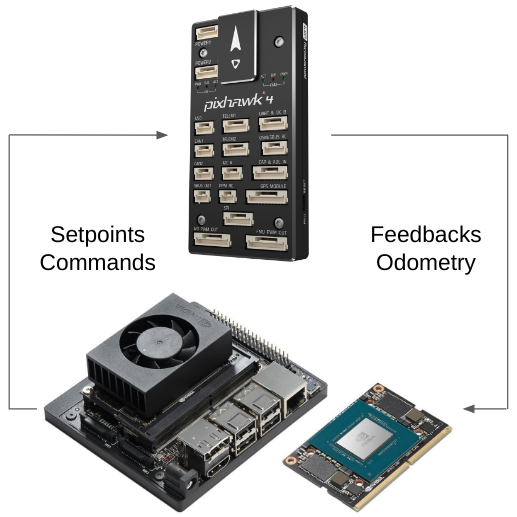
\includegraphics[width=.5\textwidth]{images/ch5/ldc21_hwarch.png}
  \caption{Functional diagram of a hardware architecture for autonomous flight: a Pixhawk 4 flight management unit (FMU) (top), and an Nvidia Jetson Xavier NX SBC (bottom).}
  \label{fig:ldc21hwarch}
\end{figure}

The flight management unit (FMU) is usually capable of passing all the necessary data to the companion computer, such as the drone's attitude, position, and velocity, as well as the status of the sensors and the actuators. The companion computer can then use this data to perform its tasks and send the commands back to the FMU. From the point of view of the companion computer, the drone is essentially the FMU: there is no distinction, since all the actuation and sensing technicalities are addressed by the FMU. Recalling the introductory discussion made in \Cref{sec:prb_design_challenges}, since an autonomous drone can be viewed as an autonomous robot, it is reasonable to suppose that its software architecture still follows a hierarchical organization. The FMU offers just a set of communication channels over which data can be sent but all of the technicalities involved in parsing this data, or sending the right commands and correctly parsing their feedback to request even a simple operation remain unsolved. Demanding this task to every single software module in the higher levels of the drone's control architecture leads to a seriously flawed design, just for a simple issue: if every module can talk to the FMU at the same time, who is actually controlling the drone at any given time? It appears clear at this point that, in such a sophisticated system, an entire layer of the architecture is reserved to modules that are in charge of interfacing with the FMU, abstracting the complexities of the communication protocols and the data formats, and providing a clear and consistent interface to the higher-level modules while handling all the necessary synchronization and arbitration tasks. This is the role of the \texttt{flight\_stack} \cite{masocco_flight_stack_nodate} DUA unit, which offers these functionalities thanks to the \ROS middleware and the PX4 firmware. Currently, it supports only multicopters but support for different types of aircraft is an ongoing development, and is based on version 1.13.3 of PX4. The \texttt{flight\_stack} repository contains five \ROS packages, the main three of which are called \texttt{px4\_msgs}, \texttt{micrortps\_agent}, and \texttt{flight\_control}.

The \texttt{px4\_msgs} package comes first since it contains a set of message definitions that are used to communicate with the FMU in both directions. These definitions correspond both in terms of fields and data types with the data packets that the modules of the PX4 firmware exchange internally among themselves. Thanks to this similarity, a module of the PX4 firmware easily serializes and deserializes packets coming from a serial UART link that connects the FMU with the companion computer. This module is called the \texttt{micrortps\_client}, and it is one of the real-time tasks of PX4; its peculiarity is that it follows the same real-time data transmission protocol that is implemented as part of the DDS standard presented in \Cref{sec:dds}. The other end of this communication is a task that runs on the companion computer, implemented as a \ROS node in the \texttt{micrortps\_agent} package. The operational task that this node performs is that of managing the serial interface connected to the FMU and interfacing it with the \ROS domain. For every different function of the PX4 firmware, there is a dedicated pair of message type and \ROS topic that the FMU either publishes or subscribes to. To make this possible, the \texttt{micrortps\_agent} node publishes or subscribes to the same \ROS topics that it offers as communication interfaces towards the FMU to other \ROS nodes running on the companion computer, handling FMU data serialization and deserialization as well as managing the serial UART link. To efficiently interface itself with the physical layer, as well as with \ROS, the \texttt{micrortps\_agent} makes use of both \ROS RMW and bare DDS APIs at the same time, the latter of which are provided by the eProsima Fast DDS implementation \cite{eprosima_fast_nodate}.

Having available a set of \ROS topics that expose all the functionalities of the PX4 firmware solves only the first half of the problem: abstracting the serial communication link and its technicalities, like message queueing and flow control, and translating it into a set of publish-subscribe communication primitives. What remains to be addressed is the abstraction of the whole drone, offering to the higher layers of the control architecture only a set of communication primitives which may even be more sophisticated than simple message topics but still hides a lot of complications concerning the execution of elementary tasks that the drone performs such as, \emph{e.g.}, takeoff and movement. This is the purpose of the \texttt{flight\_control} package, which is the core of the \texttt{flight\_stack} DUA unit.

In the control architecture of an autonomous drone, the \texttt{flight\_control} node is the first one that does not directly interface any hardware: to it, thanks to the first abstraction provided by the \texttt{micrortps\_agent}, the drone appears as another node in the architecture that communicates over a set of topics. The first, basic functionalities that the \texttt{flight\_control} offers are in fact based on this communication primitive: other nodes are expected to exchange data directly with the \texttt{flight\_control} using standard formats and it then translates the data into formats that PX4 expects and forwards the packets to the \texttt{micrortps\_agent}, which is in charge of sending them to the FMU on the serial link. Such first basic functionalities, all implemented with topics, include the following.
\begin{itemize}
  \item Position control, which is implemented by forwarding local position setpoints to PX4: nodes can send a setpoint in the form of a \ROS message, and the \texttt{flight\_control} translates it into a PX4 message and forward it to the FMU; note that this is also how hovering of a multicopter is achieved, since the \texttt{flight\_control} retains and republishes the most recent position setpoint at a frequency that avoids triggering PX4 failsafes.
  \item Velocity control, which is implemented by forwarding twist setpoints in body frame to PX4.
  \item Local pose data forwarding, for navigation in GNSS-denied environments or when an additional source of local position and orientation data is available and provided to PX4. This data has first to be transformed in a NED (North-East-Down) frame and then forwarded to PX4.
  \item PX4 local pose estimate republishing.
  \item Battery monitoring.
  \item PX4 log message monitoring.
\end{itemize}
More sophisticated functions are implemented using services and actions, that other nodes in the architecture can call acting as clients to request them and wait for their completion, receiving feedbacks in the meantime. These functions include the following.
\begin{itemize}
  \item Arming.
  \item Disarming.
  \item Takeoff.
  \item Landing.
  \item Basic movement to a specific position.
  \item Turn to a desired heading at the current position.
  \item FMU reboot.
\end{itemize}
For each of these functions, the \texttt{flight\_control} action and service servers exchange data with specific topics handled by the \texttt{micrortps\_agent}, gathering feedback and handling all possible outcomes and error conditions. In addition, the \texttt{fligth\_control} node also internally keeps track of the current operational state of the drone to allow every client to request only the operations that are possible in the current state. The \texttt{flight\_control} node is also in charge of handling the synchronization of the requests that it receives, to avoid that multiple clients request conflicting operations at the same time, and to ensure that the drone is always in a consistent state.

The relevant portion of the \texttt{flight\_stack} within the context of this work is its configuration as a DUA unit. It currently supports, and has been tested with, multiple targets ranging from SBC ones such as \texttt{jetson5}, to development ones such as \texttt{x86-cudev}. The unit configuration section of the Dockerfile for the \texttt{jetson5} target, intended for Nvidia Jetson SBCs presented in \Cref{sec:dua_supported_platforms_sbc}, is shown in \Cref{lst:flightstack}. Since no firmware development is performed on the SBC, the only configurations required concern the dependencies that are necessary for the \texttt{micrortps\_agent} to work. These include some Python packages, as well as an installation of the Fast-DDS-Gen tool by eProsima \cite{eprosima_fast-dds-gen_nodate}: this is required to generate IDL files that define messages for both the ROS and the serial side of the communications that the \texttt{micrortps\_agent} handles.

Development targets add to the aforementioned dependencies additional setup steps that configure what is required to build the PX4 firmware. For reference, \Cref{lst:flightstackdev} in \Cref{app:units} reports the unit configuration of the \texttt{x86-cudev} target. More dependencies are installed which are necessary to build the NuttX RTOS \cite{apache_software_foundation_apache_nodate}, which is the preferred real-time operating system to run the PX4 firmware on Pixhawk boards. Furthermore, since a cross-compiler is required to build the firmware in an x86 environment, version 9 of GCC \cite{free_software_foundation_gcc_nodate} for ARM is downloaded and decompressed. Finally, version 2.10.1 of eProsima Fast DDS and its dependencies are downloaded and built from source, to provide support for the compilation of the PX4-side of the communication protocol that the \texttt{micrortps\_agent} handles.

The \texttt{flight\_stack} DUA unit is a clear example of how DUA can be used to solve the integration issues that arise when developing software for autonomous systems. Focusing on the development targets, the initial dependencies are easily installed since they are distributed as packages for the system package manager and thus may be made part of the host system installation. The latter tools, however, are built from source and then installed system-wide, a process that may only be scripted at best. In contrast, DUA automates these integration and setup steps in a way that is transparent to the developer who, to use this unit, only needs to add it configuring their project targets as described in \Cref{sec:dua_template_configuration}.

\begin{center}
\begin{minipage}[t]{.9\textwidth}
\begin{lstlisting}[caption={Unit configuration of the \texttt{jetson5} target of the \texttt{flight\_stack} DUA unit \cite{masocco_flight_stack_nodate} as of November 26, 2024.}, label={lst:flightstack}]
# flight_stack START #
# Install PX4 general dependencies required by microRTPS Bridge
RUN apt-get update && apt-get install -y --no-install-recommends \
  astyle \
  libxml2-dev \
  libgstreamer-plugins-base1.0-dev \
  rsync && \
  rm -rf /var/lib/apt/lists/* /tmp/* /var/tmp/*/apt/lists/*

# Install PX4 Python dependencies required by microRTPS Bridge
RUN . /opt/dua-venv/bin/activate && yes | pip3 install -U \
  future \
  jinja2>=2.8 \
  jsonschema \
  kconfiglib \
  lxml \
  psutil \
  pygments \
  pymavlink \
  pyulog

# Build and install Fast-DDS-Gen (required by microRTPS Bridge)
WORKDIR /opt
RUN git clone --recursive --single-branch --branch 'v2.4.0' \
  https://github.com/eProsima/Fast-DDS-Gen.git && \
  cd Fast-DDS-Gen && \
  ./gradlew assemble && \
  ln -s /opt/Fast-DDS-Gen/scripts/fastddsgen scripts/fastrtpsgen && \
  cd .. && \
  chgrp -R internal Fast-DDS-Gen && \
  chmod -R g+rw Fast-DDS-Gen
WORKDIR /root
ENV PATH=/opt/Fast-DDS-Gen/scripts:${PATH}
# flight_stack END #
\end{lstlisting}
\end{minipage}
\end{center}

\subsection{Driving a sensor: zed\_drivers}
\label{sec:dua_modules_zed_drivers}
One of the hardest problems that autonomous robots face is that of localization: determining continuously its position and orientation (\emph{i.e.}, its \emph{pose}) within the environment. Robots are equipped with sensors, whose variety ranges from inertial measurement units to cameras, LiDARs, and GNSS receivers. These devices provide data that can later be used, either directly or by appropriate post-processing algorithms, to obtain an estimate of the current pose of the robot. The most common approach is that of sensor fusion, which consists of combining the data from multiple sensors to obtain an estimate of the robot's pose.

Among the many classes of sensors, RGB (Red-Green-Blue) cameras are one of the most versatile and widely used in robotics. They can range from cheap and lightweight solutions including, \emph{e.g.}, a single optic and producing only a video stream, to more expensive but sophisticated ones that include more optics and can provide additional information, such as depth maps. One of the most famous series of cameras aimed at robotics applications is the ZED series by Stereolabs \cite{stereolabs_stereolabs_nodate}. The ZED cameras are stereoscopic cameras, \emph{i.e.}, they mimic the human eye by housing two identical optics that are separated by a fixed, known distance. The sensors on each optic are synchronized, thus the frames they produce can be used to compute a depth map of the scene that the camera is viewing. This depth map can be expressed in a variety of formats, from grayscale images to point clouds, and can be employed in a variety of contexts, from obstacle avoidance to 3D environment mapping. ZED cameras have emerged as a solution also due to their software support offered by Stereolabs: the ZED SDK \cite{stereolabs_zed_nodate}. It is a versatile software development kit that enables programmers to easily interface with a ZED camera and get its data. One of the most famous disadvantages of working with images in real-time is the high cost in terms of computational power that is demanded to the host system: processing pictures usually requires a lot of memory and CPU power, and the more complex is the processing, the more resources are needed. The ZED SDK, however, has been designed to take advantage of Nvidia GPU devices present on the host, being it either a desktop computer or an SBC: thanks to the CUDA parallel computing platform, the internal algorithms of the ZED SDK can run in real-time and produce high-quality results even on low-power SBCs and similar devices. Thanks to this feature, the ZED SDK integrates a positional tracking module that, if activated, provides a real-time estimate of the pose of the camera in the environment, with respect to a reference frame that is placed at the camera's starting position. This estimate is obtained internally by the SDK algorithms by fusing the data from the camera's optics and the IMU.

In the context of a robotic software architecture based on \ROS, the integration of a sensor like a ZED camera requires the development of a specific module that abstracts it and publishes its data to the ROS network in standard formats. Such a module is usually called, in the ROS world, a \emph{driver node}: note that it is not a device driver but rather a software module that interfaces with a device and exposes its functionalities to the rest of the software architecture. It is called \emph{driver} because its task is that of of making the device work and of providing a clear and consistent interface to the rest of the nodes in the architecture, who should not be concerned with the technicalities of the device itself. The code of the driver node is based on the SDK of the device itself, if any, which is the ZED SDK in the case of the package discussed in this section: the \texttt{zed\_drivers} package \cite{masocco_zed_drivers_nodate}.

Like the other software modules discussed so far, \texttt{zed\_drivers} is a DUA unit that contains multiple \ROS software packages. The main package is called \texttt{zed\_driver} and it is the subject of the current discussion. To briefly introduce it, consider first the task that the corresponding node has to perform: a ZED camera is a hardware device that must first be opened, specifying a set of configuration parameters for its various functions, then started, and finally its data may be read, processed, and published to the \ROS network. This is, in essence, a summary of the structure of the \texttt{zed\_driver} node implemented by the package.

At startup, the \ROS node parses its parameters: these specify many configuration options of the supported functionalities of the camera, ranging from resolution and framerate, to depth sensing mode and depth map size, to IMU sampling rate. The node then initializes the ZED camera, setting it up according to the options that the parameters specified, and starts it. The node then enters a loop where it reads the data produced by the camera. The data can be divided in four main categories: RGB frames, depth maps, positional tracking data, and IMU samples. Each of these four sets of data has to be processed before it can be published over the \ROS network, mainly because it has to be copied from the program memory to properly-formatted \ROS messages that encode standard sensor data types. To streamline execution, the \texttt{zed\_driver} node runs four parallel threads that handle each type of data separately at the same time, optimizing the use of system resources to reduce latencies and ensure that the data is published before the camera produces the next frames, so that the node can keep up with the camera's framerate; the IMU thread, in particular, runs at a higher frequency sampling the camera IMU independently of the optics, since it runs at a higher rate. RGB frames have to be converted to \ROS image messages, depth maps to point cloud messages, positional tracking data to pose messages and transformations, and IMU samples to IMU messages. The node then publishes these messages over appropriate topics.

To summarize the node's capabilities, here are the ZED SDK functionalities that it supports, each with a complete set of configuration options exposed as node parameters.
\begin{itemize}
  \item RGB video stream.
  \item Depth maps and point clouds computation.
  \item IMU sampling.
  \item Pose estimation with the positional tracking module.
  \item Raw camera data logging in SVO files.
  \item Real-time video stream over the network with NVENC encoding \cite{nvidia_nvidia_nodate-1}.
\end{itemize}
To achieve this, the code of the node makes wide use of the ZED SDK C++ API. Coming back to the scope of this work, this means that a compatible installation of the ZED SDK has to be present on the host system to which the camera is connected. According to the official documentation, setting it up is easy since it is distributed as a script that first installs the dependencies and then the SDK itself. The system on which the script is run has to meet a certain set of requirements: it has to be a Ubuntu \cite{canonical_ubuntu_nodate} system with some dependencies already in place and it must have a Nvidia GPU with a version of the CUDA toolkit \cite{nvidia_cuda_nodate-1} installed which is also compatible with the version of the ZED SDK that one is installing. In the case of Jetson SBCs, things get more complicated because additional libraries, distributed by Nvidia via the JetPack SDK installation, are required. The \texttt{zed\_drivers} DUA unit automates all these setup steps, making the installation of the ZED SDK and the configuration of the project repository a matter of minutes.

Before delving into two example unit configuration Dockerfiles, recall that the system environments offered by DUA base units are stable and configured in a way to offer a good set of system packages that are ensured to be compatible with each other. Still, to install an SDK that is distributed as a self-installing script, one has to do some level of work on each target to ensure that the installation runs smoothly in a reproducible way and that it actually results in a usable SDK.

The \texttt{zed\_drivers} unit supports only targets aimed at systems that may have an Nvidia GPU. \Cref{lst:zeddriversjetson5} shows the unit configuration for the \texttt{jetson5} target. In this case, the setup is pretty straightforward: after an initial set of system dependencies that the SDK installer necessarily expects, the ZED SDK installation script is downloaded and executed. Note that, due to a compatibility issue with an Nvidia library, the version that is downloaded supports a higher JetPack version than the one on which the base unit is based: this is one of the many kinds of integration issues that usually happen in this field and that, to be solved, might require many reinstallation or board reflashes. The DUA framework, on the other hand, grants the developer the possibility to make many quick subsequent attempts without the need to reflash the Jetson board each time, by simply modifying the Dockerfile and rebuilding the image. The only critical configuration step is then the creation of a fake \texttt{/etc/nv\_tegra\_release} file that the SDK installer expects to find to correctly identify the system on which it is running, which apperas to be missing in Nvidia JetPack Docker images.

The unit configuration for the \texttt{x86-cudev} target is shown in \Cref{lst:zeddriversx86cudev}: surprisingly, this is more intricate than the one for the Jetson boards. First, due to other incompatibilities with the contents of the official Nvidia image, cuDNN \cite{nvidia_cuda_nodate} and cuBLAS libraries have to be upgraded to the latest version, the latter of which even requires a manual installation from the contents of its system package. Then, finally, the ZED SDK can be installed by downloading its installer script and running it, requiring no additional steps.

At the end of this section, after these units have been discussed as examples of how the DUA framework can help solve integration issues and provide replicable and reliable development environments, it is possible to note that thanks to the contents of these units a working prototype of an autonomous system such as an autonomous drone can be set up in a matter of minutes: first, a DUA project has to be created, adding the units to it and configuring supported targets as illustrated in \Cref{sec:dua_template_configuration}. Then, the project can be deployed onto a compatible SBC to be installed on the prototype and what is left to be done is just to download the base unit image and build the target image on top of it. A development image is then also set up to build and flash the microcontroller firmware. The necessary software modules are then ready to be built, configured, and run on the SBC, and the prototype may be tested right away.

\begin{center}
\begin{minipage}[t]{.9\textwidth}
\begin{lstlisting}[caption={Unit configuration of the \texttt{jetson5} target of the \texttt{zed\_drivers} DUA unit \cite{masocco_zed_drivers_nodate} as of November 26, 2024.}, label={lst:zeddriversjetson5}]
# zed_drivers START #
# Install ZED SDK dependencies
# (Nvidia stuff should already be installed in the base unit)
RUN apt-get update && \
  apt-get install -y --no-install-recommends \
  apt-transport-https \
  udev \
  zstd && \
  rm -rf /var/lib/apt/lists/* /tmp/* /var/tmp/*/apt/lists/*

# Install the ZED SDK
# We currently support version 4.1
# Do some more black magic here to enable streaming features
# on Jetson inside a container.
# The syntax for the echo is:
# R${L4T_MAJOR_VERSION} (release), \
#   REVISION: ${L4T_MINOR_VERSION}.${L4T_PATCH_VERSION}
# NOTE: We install an SDK version for a newer version of JetPack
# than that of this base image, due to an incompatibility with the
# deprecated libnvbuf.
RUN echo "# R35 (release), REVISION: 2.1" > /etc/nv_tegra_release && \
  wget --no-check-certificate -nc -O zed_sdk.run \
  https://download.stereolabs.com/zedsdk/4.1/l4t35.4/jetsons && \
  chmod +x zed_sdk.run && \
  ./zed_sdk.run -- silent skip_python && \
  rm zed_sdk.run && \
  ln -sf /usr/lib/aarch64-linux-gnu/tegra/libv4l2.so.0 \
  /usr/lib/aarch64-linux-gnu/libv4l2.so && \
  rm -rf /var/lib/apt/lists/* /tmp/* /var/tmp/*/apt/lists/* && \
  chgrp -R internal /usr/local/zed && \
  chmod -R g+rwx /usr/local/zed
ENV LD_LIBRARY_PATH=${LD_LIBRARY_PATH}:/usr/local/zed/lib
ENV LOGNAME=neo
# zed_drivers END #
\end{lstlisting}
\end{minipage}
\end{center}

\begin{center}
\begin{minipage}[t]{.9\textwidth}
\begin{lstlisting}[caption={Unit configuration of the \texttt{x86-cudev} target of the \texttt{zed\_drivers} DUA unit \cite{masocco_zed_drivers_nodate} as of November 26, 2024.}, label={lst:zeddriversx86cudev}]
# zed_drivers START #
# Install ZED SDK dependencies
# NOTE: Here we require an upgrade to make sure
# we have the latest Nvidia libraries.
RUN apt-get update && apt-get install -y \
  --no-install-recommends --allow-change-held-packages \
  libcudnn8 \
  libcudnn8-dev \
  zstd && \
  rm -rf /var/lib/apt/lists/* /tmp/* /var/tmp/*/apt/lists/*

# Install libcublas-12-0 libraries manually
# to fix some incompatibilities in ZED SDK dependencies
WORKDIR /tmp
RUN apt-get update && \
  apt-get download libcublas-12-0 && \
  mkdir contents && \
  dpkg-deb -xv libcublas-12-0_12.0.2.224-1_amd64.deb contents/ && \
  mv contents/usr/local/cuda-12.0/targets/x86_64-linux/lib/* \
  /usr/local/cuda/lib64/ && \
  rm -rf contents libcublas-12-0_12.0.2.224-1_amd64.deb && \
  ldconfig && \
  rm -rf /var/lib/apt/lists/* /tmp/* /var/tmp/*/apt/lists/*
WORKDIR /root

# Install the ZED SDK
# We currently support version 4.1
RUN wget -nc -O zed_sdk.run \
  https://download.stereolabs.com/zedsdk/4.1/cu118/ubuntu22 && \
  chmod +x zed_sdk.run && \
  ./zed_sdk.run -- silent skip_python && \
  rm zed_sdk.run && \
  rm -rf /var/lib/apt/lists/* /tmp/* /var/tmp/*/apt/lists/* && \
  chgrp -R internal /usr/local/zed && \
  chmod -R g+rwx /usr/local/zed
ENV LD_LIBRARY_PATH=${LD_LIBRARY_PATH}:/usr/local/zed/lib
# zed_drivers END #
\end{lstlisting}
\end{minipage}
\end{center}

\section{Preliminary results}
\label{sec:robots_results}
The DUA framework and the technologies presented so far have led to the development of a few prototypes during the time in which this thesis was drafted. These prototypes were developed either to perform specific tasks in real-world scenarios, or to test novel solutions in fields like robot autonomy and localization and mapping. The common ground of these prototypes is the use of the DUA framework in their development and deployment, which proved the effectiveness of the proposed solutions. This section presents some preliminary published results concerning the application of the technologies on which DUA is based to the field of autonomous robotics. Their success has brought to the formalization of the DUA framework as presented in \Cref{ch:dua}, as well as to the solutions presented in the previous \Cref{sec:dua-utils}.

\subsection{A \ROS distributed architecture for unmanned aircraft}
\label{sec:robots_results_paperdrone2021}
In \cite{bianchi_novel_2023}, a novel distributed architecture is designed and proposed for an autonomous drone, tasked with the execution of a target reconnaissance and precision landing mission in an indoor, GNSS-denied environment. The mission was part of the 2021 Edition of the Leonardo Drone Contest, a robotics competition hosted by Leonardo S.p.A. in which custom-built UASs have to perform a series of complex tasks autonomously, ranging from localization and flight control to environment mapping and autonomous navigation.

The research team from the Tor Vergata University of Rome participated in the 2021 Leonardo Drone Contest, which was conducted in Turin, Italy during September 2021. This competition featured six Italian universities deploying autonomous drones to execute a sophisticated mission within a structured indoor environment. The operational field was meticulously configured with various elements, including 10 distinct landing pads and 3 mobile ground robots, with all participants receiving comprehensive details about the field layout prior to the competition. The visual markers demarcating the landing pads provided additional navigational guidance. A depiction of the 2021 field layout is shown in \Cref{fig:ldc21field}: landing pads are in green and marked with their numerical ID, while known obstacles are in gray and their height in centimeters is reported.
\begin{figure}[t!]
  \centering
  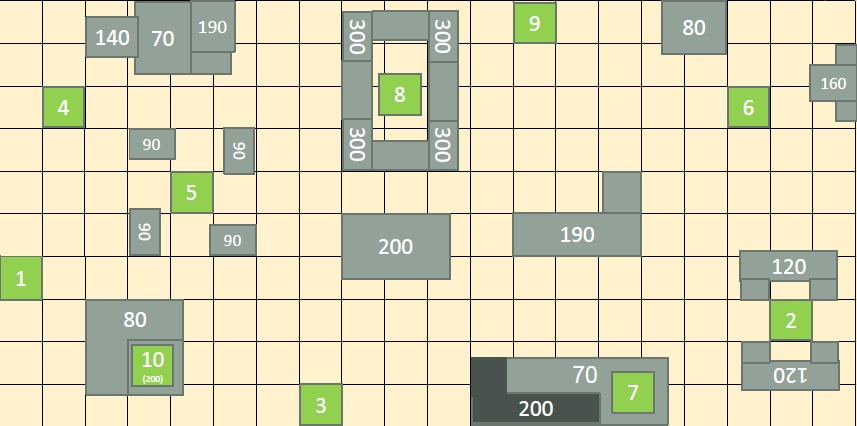
\includegraphics[width=.8\textwidth]{images/ch5/ldc21_field.jpg}
  \caption{The 2021 Leonardo Drone Contest field layout.}
  \label{fig:ldc21field}
\end{figure}

The mission objectives for each drone were structured as follows.
\begin{enumerate}
  \item Initiate take-off from a designated pad.
  \item Conduct environmental reconnaissance to locate one of the three ground-based mobile robots.
  \item Capture photographic documentation of the identified robot and transmit the imagery to an operator, who would subsequently communicate a specific landing sequence.
  \item Execute precision navigation between pads, performing sequential landings and take-offs according to the prescribed sequence.
\end{enumerate}

Participants were allowed to use a Ground Control Station (GCS) for mission initialization and continuous drone monitoring. The landing sequence was strategically determined by an operator at the GCS to optimize the cumulative score, which was calculated through the summation of points assigned to each successful landing on a given pad. The point distribution was uniquely encoded on the ground-based robot, so it required initial identification.

The competition imposed rigorous technical constraints on all participating teams. Specifically, the use of GNSS platforms was prohibited, and Light Detection and Ranging (LiDAR) sensors were expressly forbidden. Additionally, teams were precluded from deploying any fixed ground-based sensors or motion capture systems, thereby challenging participants to develop innovative autonomous navigation strategies using the few remaining sensors which were not only allowed, but also capable of being mounted on a small UAS.

To facilitate the comprehensive mission objectives, a sophisticated hardware and software architecture was meticulously designed and implemented on advanced hardware. The autonomous quadcopter developed for the Leonardo Drone Contest 2021 represents a complex system that not only meets the specified requirements but also serves as an optimal test framework for the methodologies introduced in \Cref{ch:tools}. The architectural design strategically partitions both hardware and software components across multiple hierarchical levels, addressing the distinct critical challenges inherent to each layer.

\subsubsection{Implementation details}
\label{sec:robots_results_paperdrone2021_impl}
The hardware architecture was composed by three distinct systems: a Holybro Pixhawk 4 flight controller (see \Cref{sec:dua_modules_flight_stack}), an Nvidia Jetson Xavier NX companion computer (see \Cref{sec:dua_supported_platforms_sbc}), and a PC acting as the Ground Control Station. The two embedded systems were mounted on the UAS prototype and interconnected as in \Cref{fig:ldc21hwarch}, which also depicts a functional diagram for the hardware architecture: the Pixhawk 4 flight controller is responsible for low-level flight control tasks, while the Nvidia Jetson Xavier NX companion computer executes high-level algorithms and mission-critical tasks and interfaces with the former to send commands and receive feedbacks and status data. A summary of the technical specifications of these two embedded systems is given in \Cref{tab:ldc21_sbcs}.
\begin{table}[t]
  \centering
  \begin{tabular}{|c|c|}
    \hline
    \multicolumn{2}{|c|}{\textbf{Nvidia Jetson Xavier NX}}\\
    \hline
    CPU & NVIDIA Carmel ARM v8.2 (6C/6T, up to \SI{1.4}{GHz})\\
    RAM & \SI{8}{GB} LPDDR4x\\
    GPU & NVIDIA Volta (384 CUDA Cores, 48 Tensor Cores)\\
    OS  & Ubuntu Linux 20.04\\
    \hline
    \multicolumn{2}{|c|}{\textbf{Holybro Pixhawk 4}}\\
    \hline
    CPU & STM32F765 (ARM Cortex-M7, up to \SI{216}{MHz})\\
    RAM & \SI{512}{KB}\\
    OS  & NuttX 10.0.0\\
    \hline
  \end{tabular}
  \caption{Main technical specifications of the SBCs used in the implementation.}
  \label{tab:ldc21_sbcs}
\end{table}

\Cref{fig:ldc21swarch} illustrates the comprehensive organization of software modules across functional layers.
\begin{itemize}
  \item \textbf{Lowest Layer:} Comprised of real-time modules critical for executing fundamental flight operations, as well as device drivers.
  \item \textbf{Middle Layers:} Hosts higher-level, computationally intensive algorithms responsible for executing individual mission tasks.
  \item \textbf{Highest Layer:} Dedicated to supervision logic, implemented as a Finite-State Machine (FSM), and the Ground Control Station (GCS) operator interface.
\end{itemize}
The architectural objective was to develop a cohesive set of \ROS modules that leverage interdependent functionality. This modular approach ensures vertical abstraction, enabling higher-level modules to operate without direct concern for lower-level implementation details such as take-off, landing, and navigational maneuvers. By abstracting these fundamental operations, the architecture promotes a clean, hierarchical system design that enhances modularity and operational flexibility.
\begin{figure}[t!]
  \centering
  \includesvg[width=\textwidth]{images/ch5/ldc21_swarch.svg}
  \caption{Software architecture of the LDC21 autonomous drone: thin arrows indicate communications established with \ROS interfaces, thick arrows represent dedicated software interfaces, white boxes represent \ROS nodes.}
  \label{fig:ldc21swarch}
\end{figure}

Regarding the set of software modules running on the UAS onboard computers, the lowest layer was composed of the early version of what has become the \texttt{flight\_stack} DUA unit presented in \Cref{sec:dua_modules_flight_stack}. This prototype was in fact running the very first version of this software, and it has provided a testbed for the development of a bridged DDS-based communication among the two levels of the onboard architecture.

The remaining layers contain modules that concern the following specific tasks: perception, navigation and exploration, and mission supervision. Regarding perception, the prototype was equipped with two Intel RealSense D435i depth cameras: one was pointed forward and used for localization, while the other was pointed downward and used for target detection. Both mobile robots and landing pads were equipped with ArUco markers \cite{romero-ramirez_speeded_2018,garrido-jurado_generation_2016}, a particular kind of fiducial markers with limited information aimed at improving detection probability and pose estimation capabilities. The \texttt{ArUco Scanner} module was responsible for detecting these markers and transmitting detection data to the \texttt{FSM} module, that ran a state machine to manage the mission phases and the drone behavior.

To understand the environment and get a consistent estimate of its position and orientation within it, the UAS ran a VSLAM (Visual Simultaneous Localization And Mapping) algorithm. The SLAM problem is notoriously complex and computationally intensive to solve, requiring sophisticated solutions from both the mathematical and implementation perspectives. Nonetheless, it was deemed as the only solution in this case due to the Contest rules: no sensors other than cameras were reliable enough to provide the required information, and due to accumulated error it was not possible to rely on odometry alone. The chosen VSLAM algorithm for this implementation was the ORB-SLAM2 system \cite{mur-artal_orb-slam2_2017}, a state-of-the-art solution for monocular, stereo, and RGB-D cameras that provides real-time performance and high accuracy in both localization and mapping tasks.

The \texttt{VSLAM} module was responsible for running the algorithm and providing the estimated pose of the drone directly to the PX4 firmware. The ORB-SLAM2 system employs binary feature extraction from input frames to construct a local map while addressing bundle adjustment optimization problems. To maximize computational efficiency and optimize memory utilization, these features are consistently employed throughout the entire system. The algorithm designates certain frames as keyframes, which serve as critical reference points for the local map structure. These keyframes are instrumental in computing the current local pose through the construction of a \emph{covisibility graph}, which facilitates both localization and environmental mapping functions. As the map increases in scale, the system generates an additional structural representation known as the \emph{essential graph}, which enables loop detection capabilities. Upon loop detection, the system executes an automatic loop closure procedure wherein all graphs undergo analysis and updating. During this process, redundant keyframes and nodes are eliminated, and the local map undergoes revision incorporating recent measurements to minimize systematic errors.

The architecture of the ORB-SLAM2 system comprises four distinct operational phases: tracking, local mapping, loop closing, and global adjustment. Each phase executes in a dedicated thread. The tracking phase monitors scene features, while local mapping utilizes these same features to construct the local map in relation to the established keyframes. The loop closing phase identifies potential loops and communicates this information to the global adjustment thread, which performs global bundle adjustment across the entire map to enhance overall accuracy.

ORB-SLAM2 supports multiple input modes: monocular, stereo, and RGB-D. The implementation used in this work introduces an additional mode that uses infrared and depth images, called IRD mode. This modification addresses specific technical limitations of Intel RealSense cameras, particularly the temporal misalignment between RGB and depth frames, while maintaining proper synchronization with infrared frames. Significant modifications to the ORB-SLAM2 algorithm have been implemented to expand parameter control capabilities, incorporate ARM processor compatibility, and integrate NVIDIA CUDA GPU optimizations. The adaptation for ARM architecture required the disabling of x86-specific optimizations, particularly affecting performance in feature extraction and computation phases that previously leveraged AVX/SSE vector instruction sets. To address these performance implications, CUDA GPU optimization became essential. Within the distributed architecture shown in \Cref{fig:ldc21swarch}, this algorithm operates as a \ROS node, consuming camera topic frames and publishing both the current pose estimation and system state on separate topics.

The next task to address was that of autonomous navigation and exploration of the environment, to find ground targets and landing zones. The \texttt{Navigator} module was implemented for this purpose, with the aim of providing a high-level interface to navigation operations. These operations were exposed as \ROS synchronous communication primitives, \emph{i.e.}, in the form of services: their refinement as more complex operations requiring a stateful communication was left as future work and developed for subsequent prototypes. The \texttt{Navigator} module was responsible for sending commands to the lower levels to move the drone from its current position to a given target position, provided that such a position was reachable and that there existed a path to reach it. This additional task of computing and returning paths was left to the \texttt{Path Finder} module: its primary objective was to determine an optimal trajectory between current and target positions that simultaneously minimizes distance while ensuring collision avoidance. The implemented solution approaches path planning through graph construction representing traversable space within the environment. Trajectory optimization utilizes the A* search algorithm \cite{guruji_time-efficient_2016}.

The algorithm initially constructs a graph representation directly from environmental point cloud data acquired via ORB-SLAM2. This process begins by discretizing the environment into a three-dimensional grid of variable-resolution cubic cells, each identified by its centroid. The interconnection network of traversable cells constitutes the graph structure. Boundary cells are automatically designated as non-traversable to constrain the UAS operational space. Environmental obstacle identification proceeds through point cloud preprocessing, beginning with the removal of out-of-bounds points. The algorithm associates points with their containing cells, designating cells exceeding a predetermined point density threshold as non-traversable. The remaining cells form the graph vertex set, followed by edge construction. For each cell, the algorithm identifies neighboring cells in eight coplanar directions at equal altitude, plus immediate vertical neighbors. Edge insertion between adjacent cells depends on a corridor analysis based on the physical dimensions of the drone: an edge is established if and only if the point density within the corridor falls below a specified threshold. This methodology enables variable-resolution environmental discretization while maintaining consideration for the physical footprint of the drone during transitions.

Valid corridors result in edge insertion with costs equal to the Euclidean distance between cell centroids. This iterative process yields a graph representation of the operational space, computed offline. The designated \texttt{Path Finder} \ROS node implements a computationally optimized A* algorithm to determine shortest paths between arbitrary nodes upon request, carried over a service interface. Path finding operations begin with origin and target cube identification and validation. Upon confirming traversability, the algorithm initiates shortest path computation, returning a sequence of waypoints leading to the target position. The selection of A* is motivated by its mathematical properties of admissibility, completeness, and optimality. As an informed search algorithm, A* leverages domain knowledge through heuristic guidance, distinguishing it from other similar algorithms. In the context of three-dimensional navigation, the implementation employs Euclidean distance as its heuristic function, facilitating efficient minimum-distance path identification.

\subsubsection{Supervision}
\label{sec:robots_results_paperdrone2021_supervision}
The software architecture culminates in a finite-state machine that implements high-level supervision logic. This FSM presents the drone as an automaton executing complete missions within the Leonardo Drone Contest parameters while managing contingencies such as hardware failures, battery depletion, and localization system degradation or complete failure. State transitions trigger formulation of requests to subordinate modules, with transitions conditioned upon both current state and intervening events.

The implementation integrates with the distributed architecture through a \ROS node that facilitates bidirectional communication with other modules via service calls and alert reception. System initialization comprises a comprehensive status verification of all modules through \ROS middleware APIs; mission execution begins only upon confirmation of full operational readiness across all subsystems.

The structure of the FSM mirrors mission dynamics as specified in the Contest rules. The implementation consolidates all abstraction levels into a single routine where state transitions are invoked based on the operational conditions of the drone following each execution step. Error handling leverages the meta-machine concept: primary mission phases execute within states comprising a subordinate FSM, while maintaining guaranteed transition paths to termination states under all circumstances. The high-level and low-level FSMs are shown in \Cref{fig:ldc21fsmhl,fig:ldc21fsmll}.
\begin{figure}[t!]
  \centering
  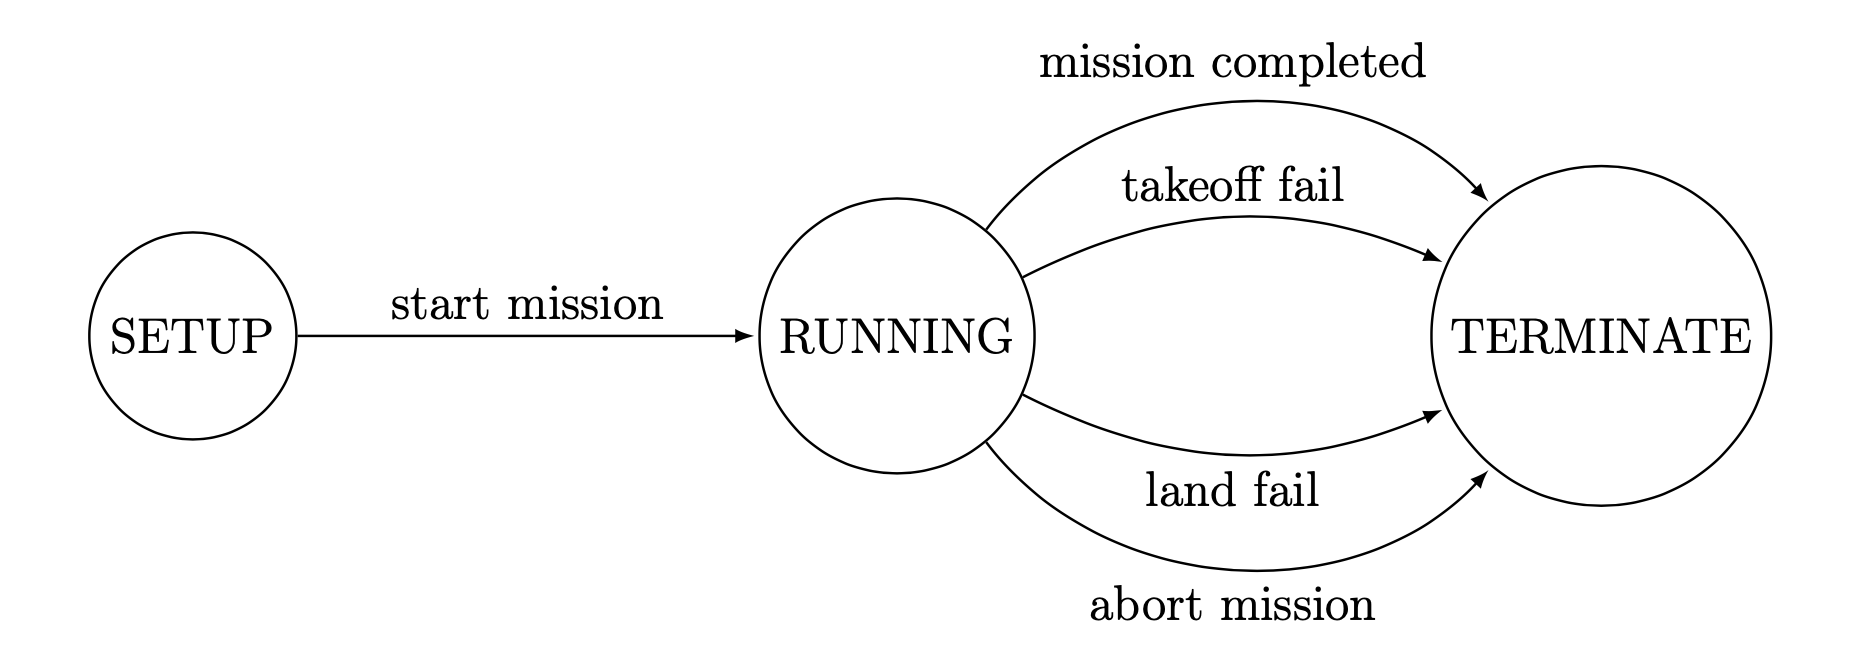
\includegraphics[width=.9\textwidth]{images/ch5/ldc21_FSM_HL.png}
  \caption{High-level finite-state machine for the Leonardo Drone Contest 2021 mission.}
  \label{fig:ldc21fsmhl}
\end{figure}
\begin{figure}[t!]
  \centering
  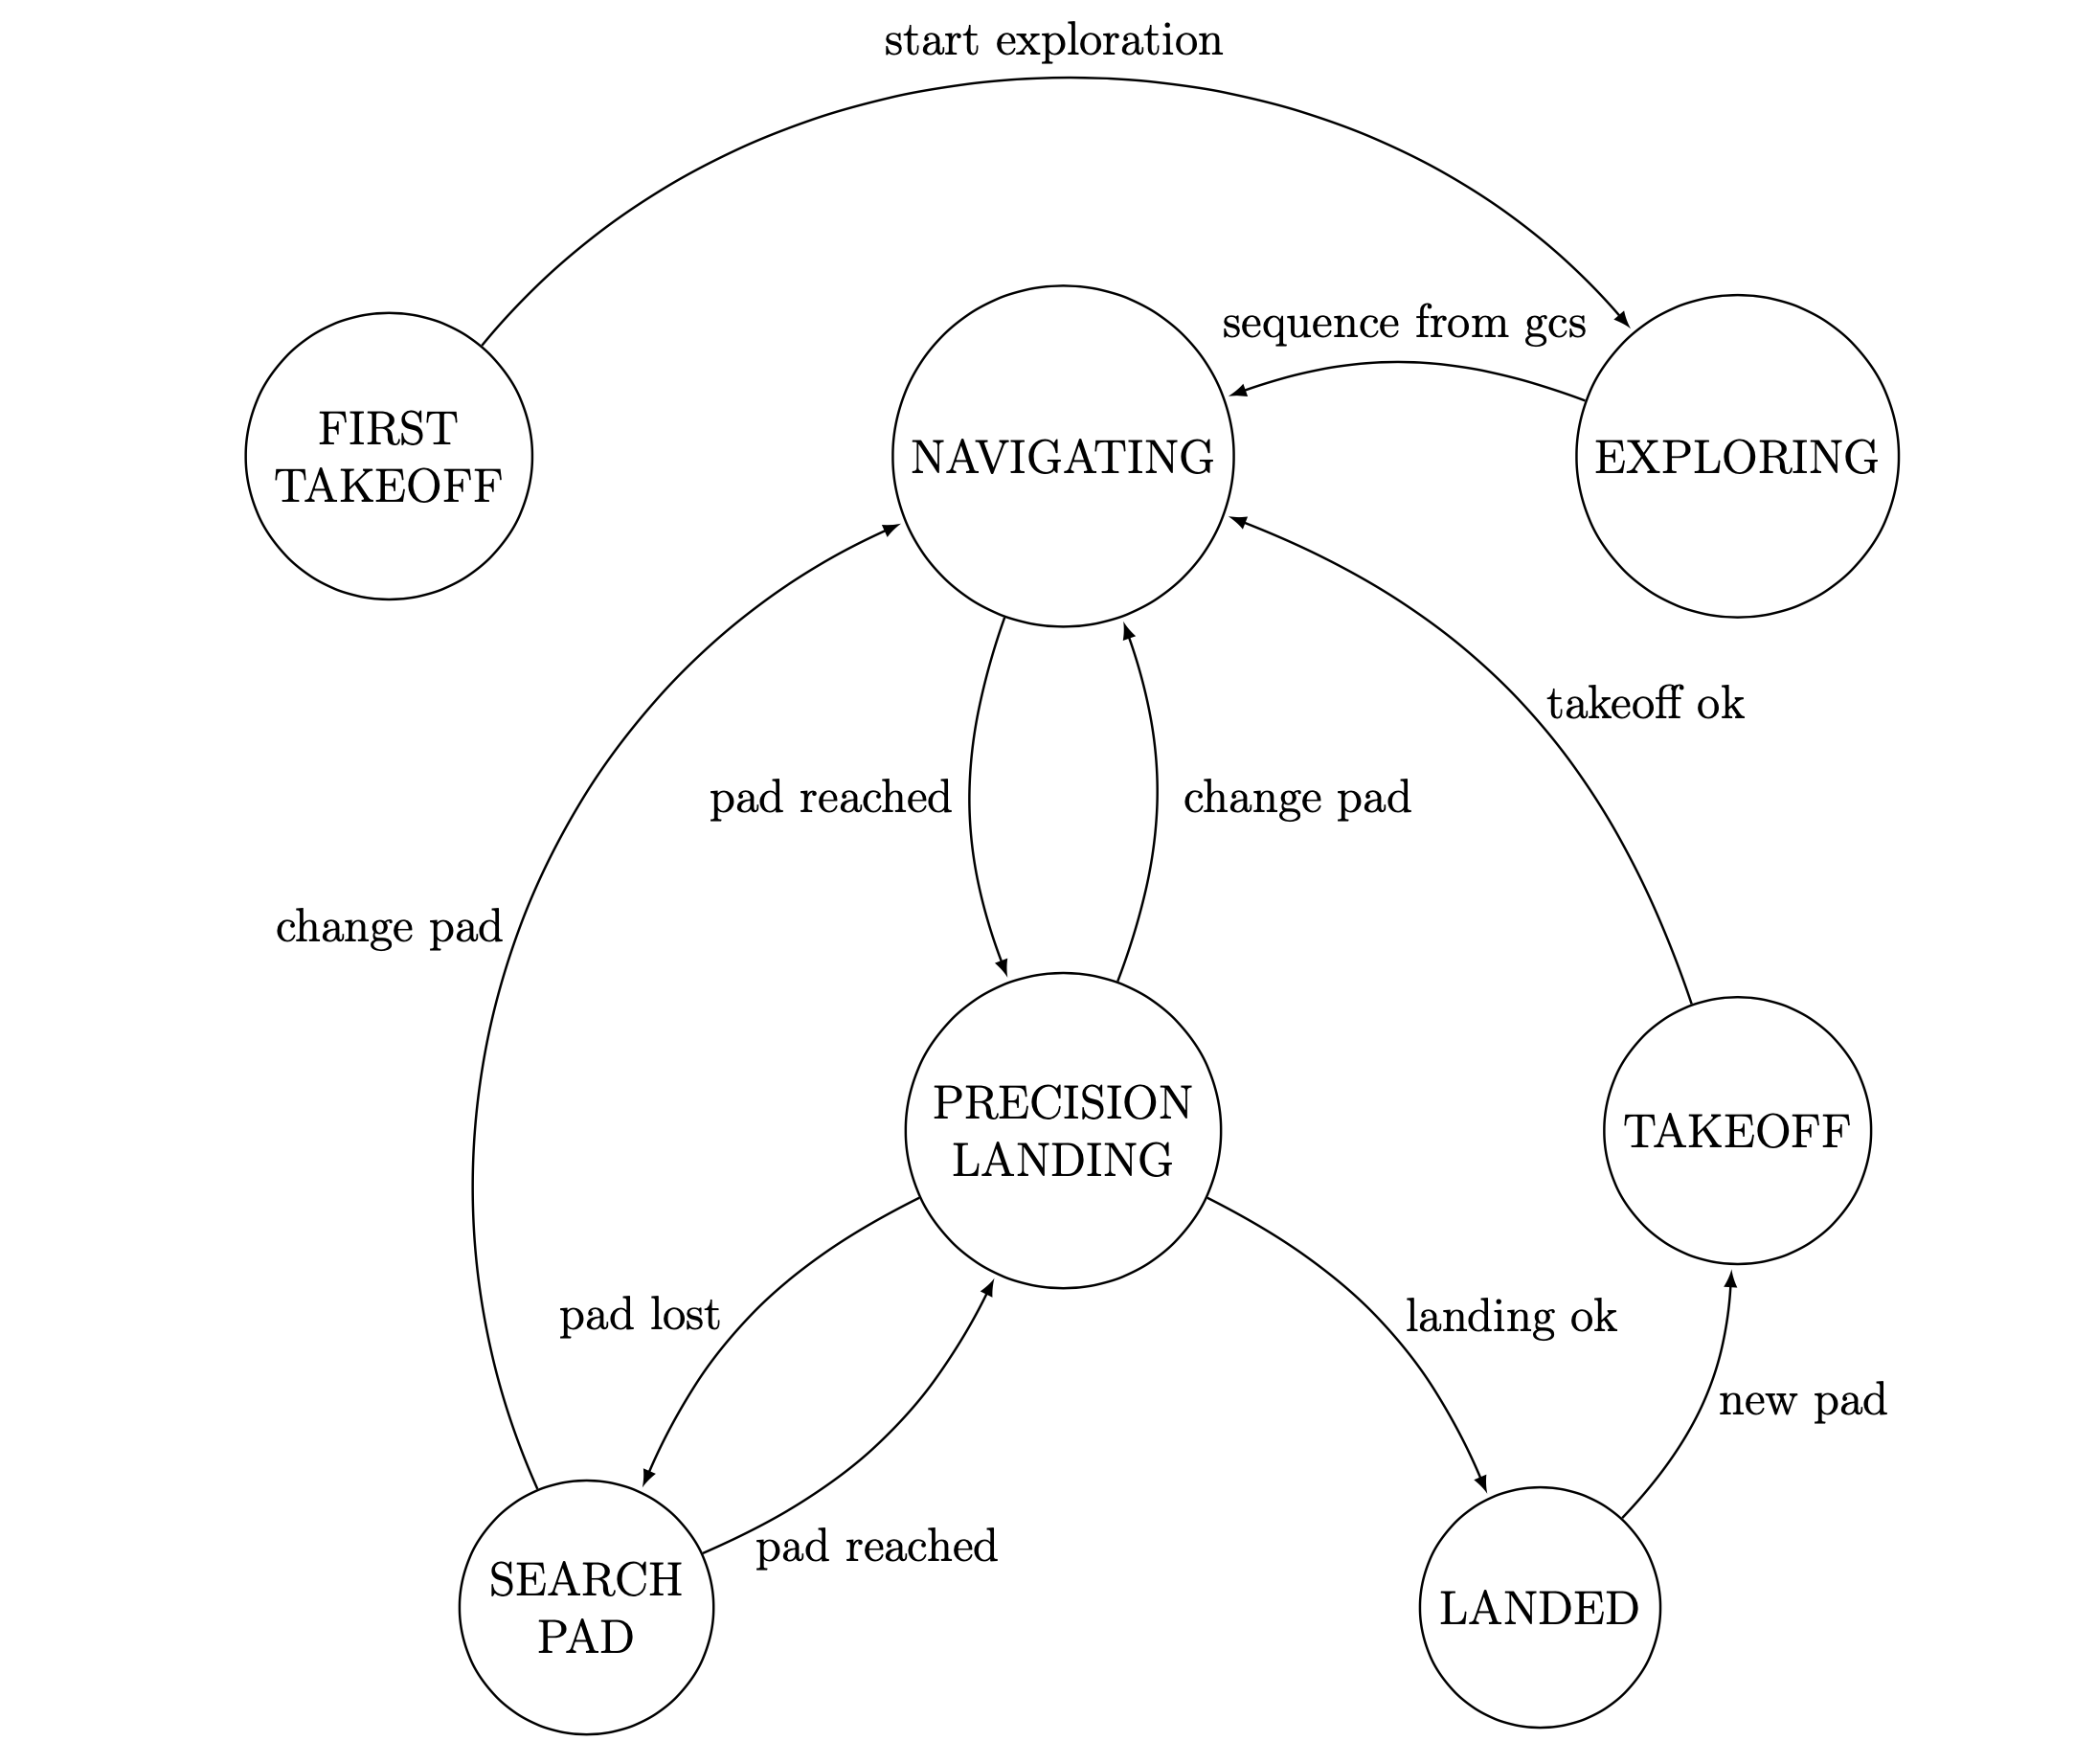
\includegraphics[width=.9\textwidth]{images/ch5/ldc21_FSM_LL.png}
  \caption{Low-level finite-state machine for the Leonardo Drone Contest 2021 mission.}
  \label{fig:ldc21fsmll}
\end{figure}

\subsubsection{Experimental results}
\label{sec:robots_results_paperdrone2021_results}

\begin{figure}[t!]
	\centering
	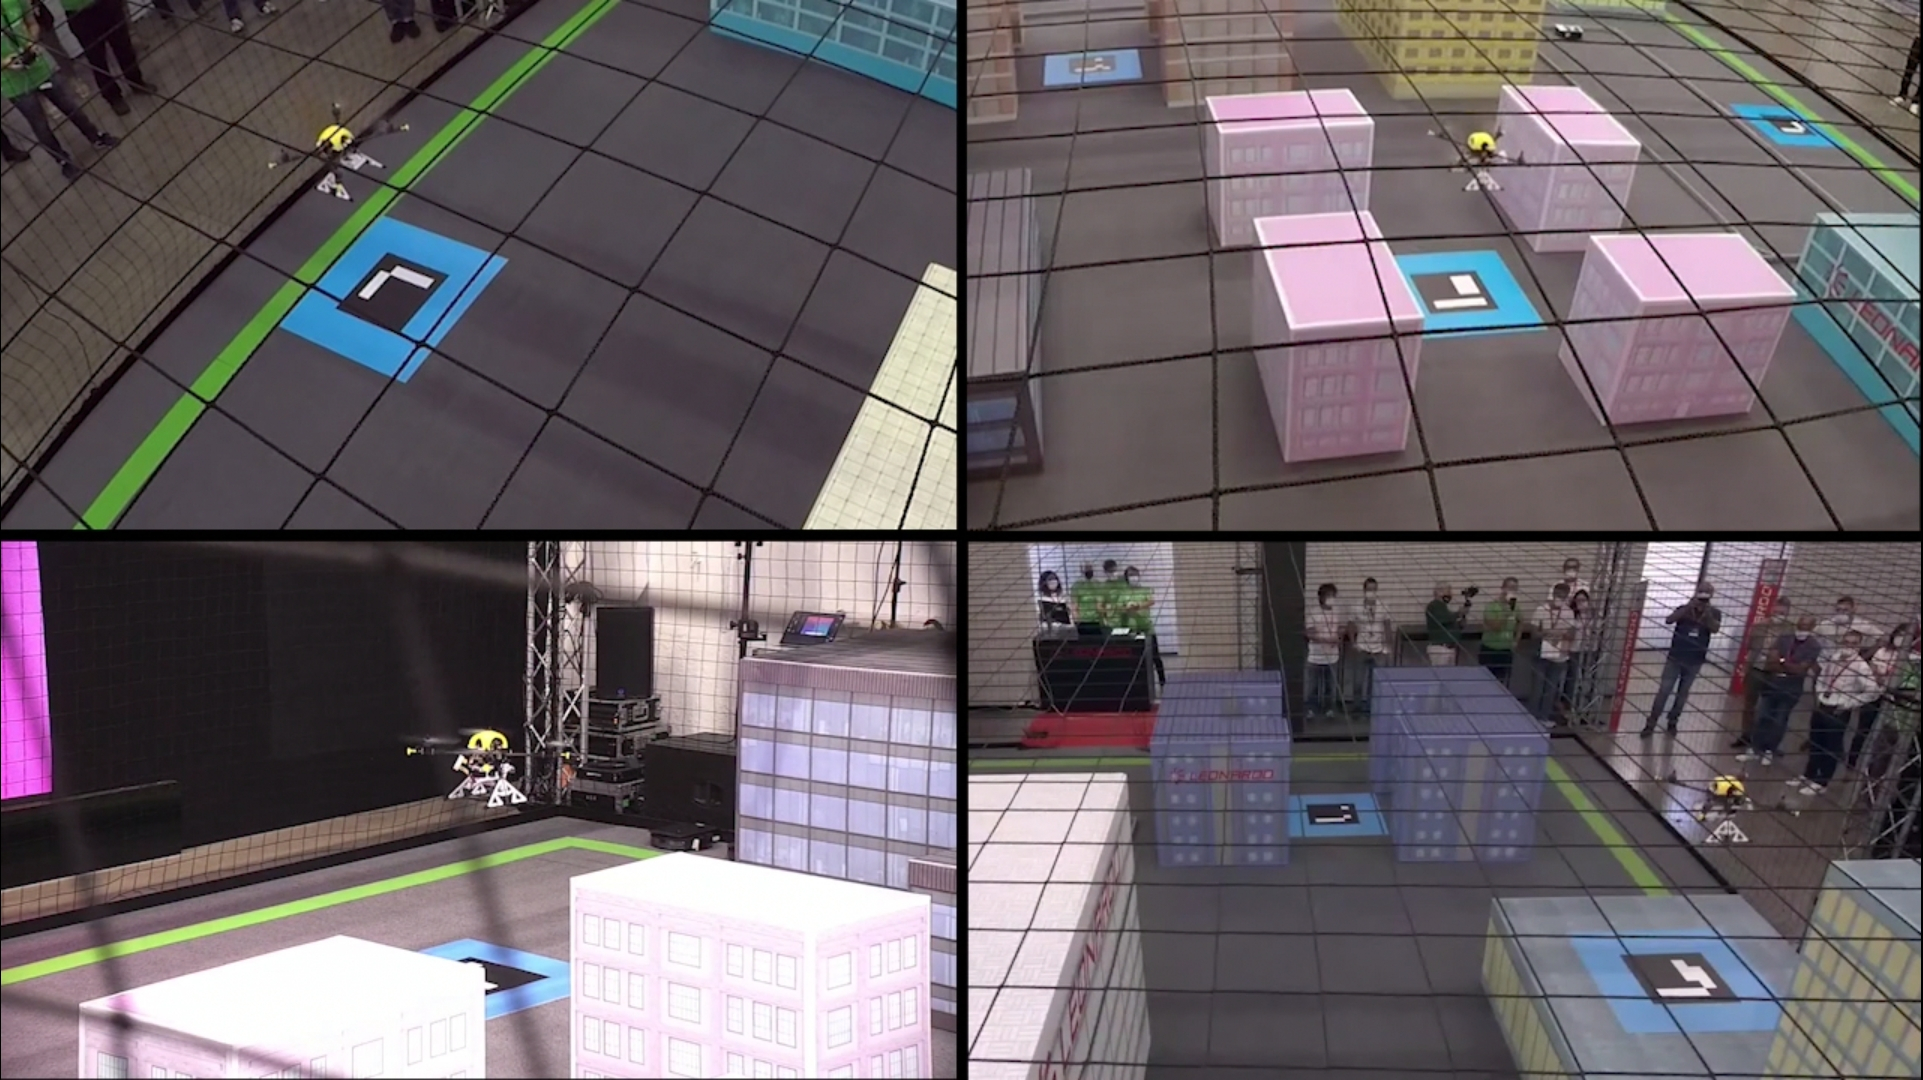
\includegraphics[width=.9\textwidth]{images/ch5/ldc21_frame1.jpg} \\
	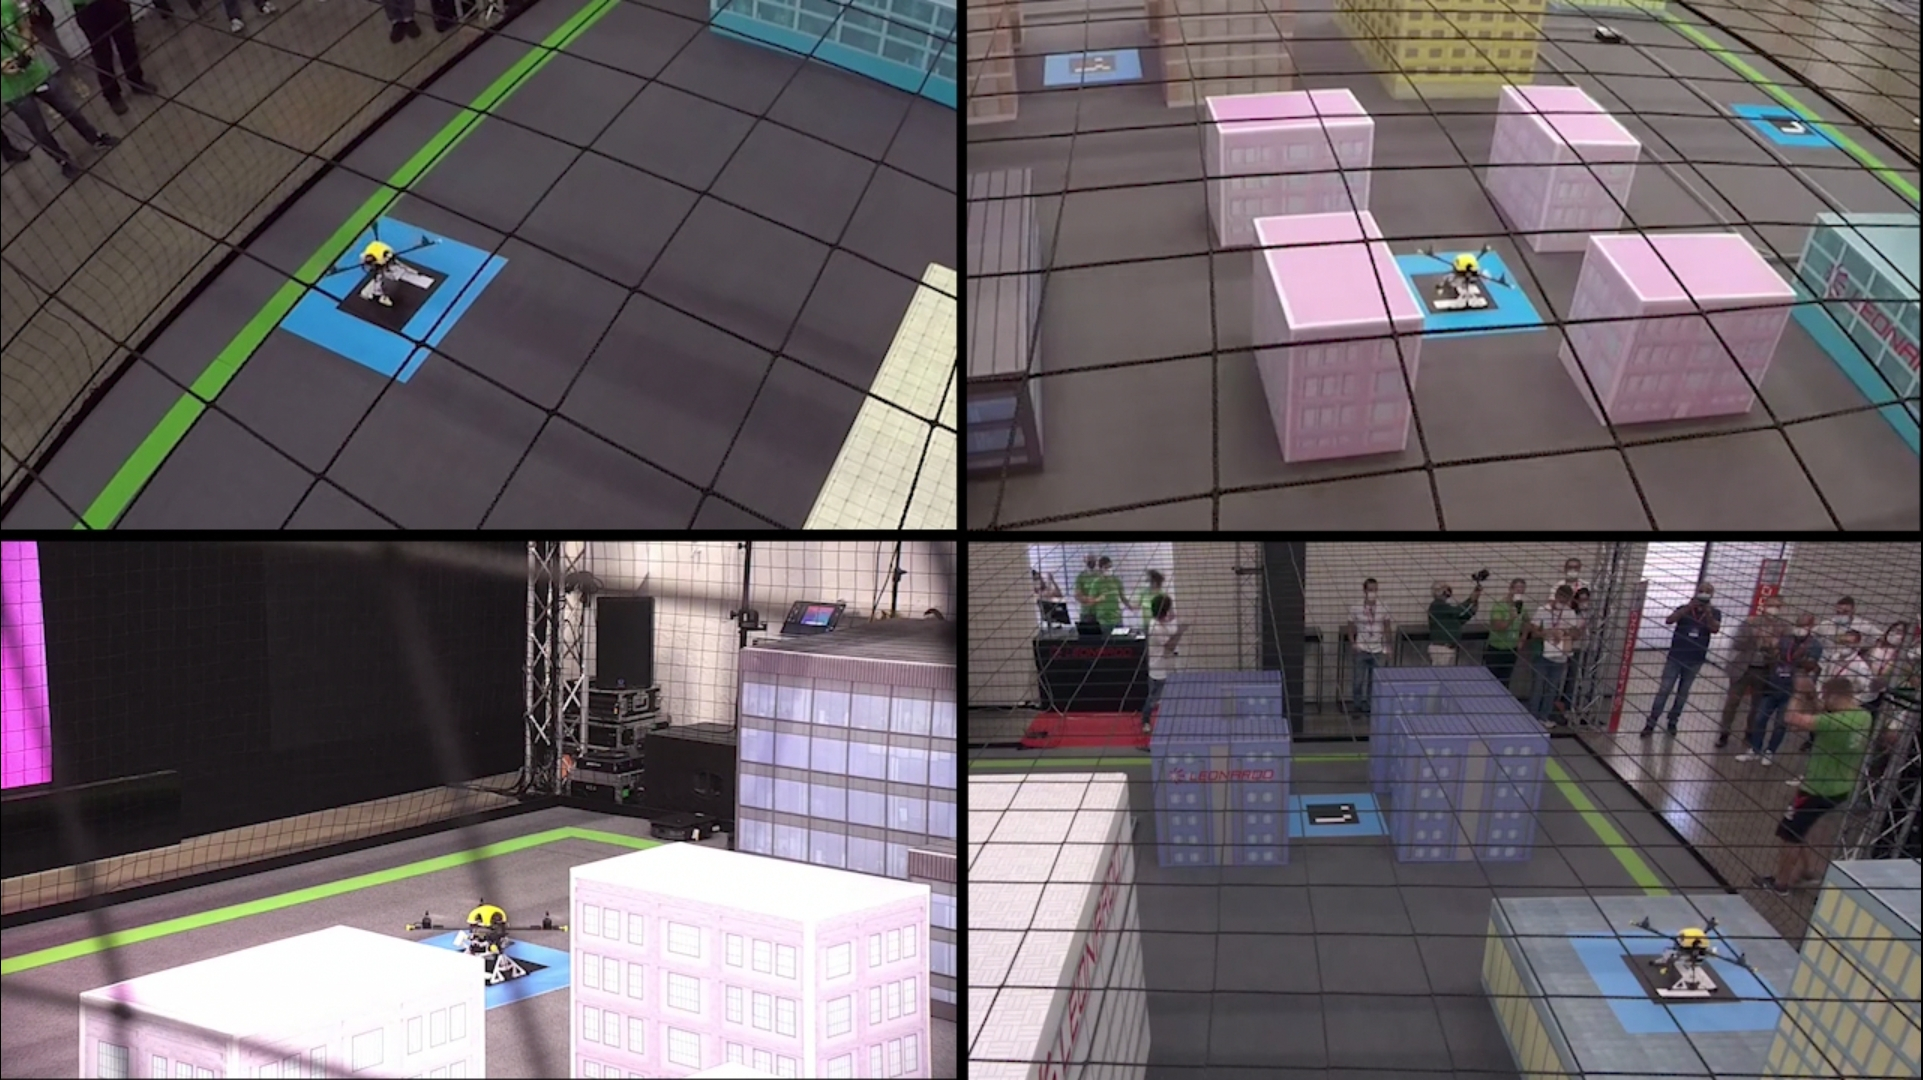
\includegraphics[width=.9\textwidth]{images/ch5/ldc21_frame2.jpg}
	\caption{Successful precision landings performed on the ArUco landing pads during the 2021 Leonardo Drone Contest.}
	\label{fig:ldc21_preclands}
\end{figure}

